%%%%%%%%%%%%%%%%%%%%%%% File template.tex %%%%%%%%%%%%%%%%%%%%%%%%%
%
% This is a general template file for the LaTeX package SVJour3
% for Springer journals.          Springer Heidelberg 2010/09/16
%
% Copy it to a new file with a new name and use it as the basis
% for your article. Delete % signs as needed.
%
% This template includes a few options for different layouts and
% content for various journals. Please consult a previous issue of
% your journal as needed.
%
%%%%%%%%%%%%%%%%%%%%%%%%%%%%%%%%%%%%%%%%%%%%%%%%%%%%%%%%%%%%%%%%%%%
%
% First comes an example EPS file -- just ignore it and
% proceed on the \documentclass line
% your LaTeX will extract the file if required
%\begin{filecontents*}{example.eps}
%!PS-Adobe-3.0 EPSF-3.0
%%BoundingBox: 19 19 221 221
%%CreationDate: Mon Sep 29 1997
%%Creator: programmed by hand (JK)
%%EndComments
%gsave
%newpath
%  20 20 moveto
%  20 220 lineto
%  220 220 lineto
%  220 20 lineto
%closepath
%2 setlinewidth
%gsave
%  .4 setgray fill
%grestore
%stroke
%grestore
%\end{filecontents*}
%
\RequirePackage{fix-cm}
%
%\documentclass{svjour3}                     % onecolumn (standard format)
%\documentclass[smallcondensed]{svjour3}     % onecolumn (ditto)
\documentclass[smallextended]{svjour3}       % onecolumn (second format)
%\documentclass[twocolumn]{svjour3}          % twocolumn
%
\smartqed  % flush right qed marks, e.g. at end of proof
%
\usepackage{graphicx}
\usepackage{tabulary}
%
%\usepackage{mathptmx}      % use Times fonts if available on your TeX system
%
% insert here the call for the packages your document requires
%\usepackage{latexsym}
%\usepackage{amsmath}
%\usepackage{amsthm}
\usepackage{array}
\usepackage{color}
\usepackage{caption}
\usepackage{float}
%\usepackage{subfigure}
\usepackage{amssymb}
\usepackage{multirow}
\usepackage{multirow}
%\usepackage{subcaption}
%MRS2: check the appropriate natbib options to give the type of citations JCAMD has (bracketed numbers)
\usepackage[numbers, square,sort&compress]{natbib}
\graphicspath{{figures/}}
%
% please place your own definitions here and don't use \def but
\newcommand{\BibTex}{\textsc{Bib}\TeX}
\newcommand{\erfc}{\mathrm{erfc}}
%
% Insert the name of "your journal" with
\journalname{JCAMD}
%
\begin{document}

\title{Lessons learned from comparing molecular dynamics engines on the SAMPL5 dataset}
%DLM: Such a long title. What about "Lessons on molecular dynamics engine comparison from SAMPL5"?
%MRS: maybe this?  I'm not so phobic about long descriptive titles, since usually that's all a person sees in a search engine.
%\thanks{Grants or other notes
%about the article that should go on the front page should be
%placed here. General acknowledgments should be placed at the end of the article.}
%\subtitle{Do you have a subtitle?\\ If so, write it here}

\titlerunning{Lessons learned from comparing molecular dynamics simulation engines}        % if too long for running head

\author{Michael R. Shirts \and Christoph Klein \and Jason M. Swails \and Jian Yin \and Michael K. Gilson \and David L. Mobley \and David A. Case \and Ellen D. Zhong}

\authorrunning{M. R. Shirts et al.} % if too long for running head

\institute{Michael R. Shirts \at
              Department of Chemical and Biological Engineering, University of Colorado Boulder,
              Boulder, Colorado, USA 
		\email{michael.shirts@colorado.edu}
           \and Christoph Klein \at
              Department of Chemical Engineering, Vanderbilt University, Nashville, TN, USA
              \and Jason M. Swails \at Department of Chemistry and Chemical Biology, Rutgers University, Rutgers, NJ, USA  % no currently there, but most of the work was performed here?  Jason, let me know what your thoughts are on this   
              \and Jian Yin \at Skaggs School of Pharmacy and Pharmaceutical Sciences, University of California, San Diego, CA, USA
              \and Michael K. Gilson \at Skaggs School of Pharmacy and Pharmaceutical Sciences, University of California, San Diego, CA, USA
              \and David L. Mobley \at Departments of Pharmaceutical Sciences and Chemistry, University of California, Irvine, Irvine, CA, USA
              \and David A. Case \at Department of Chemistry and Chemical Biology, Rutgers University, Rutgers, NJ, USA
              \and Ellen D. Zhong \at Department of Chemical Engineering, University of Virginia, Charlottesville, VA, USA % essentially all the work was done when in my group, and Shaw may have issues with their name appearing somewhere else. 
}

\date{Received: date / Accepted: date}
% The correct dates will be entered by the editor


\maketitle

\begin{abstract}

We describe our efforts to prepare common starting structures and
models for the SAMPL5 blind prediction challenge. We generated the
starting input files and single configuration potential energies for
the host-guest in the SAMPL5 blind prediction challenge for the
GROMACS, AMBER, LAMMPS, DESMOND and CHARMM molecular simulation
programs. All conversions were fully automated from the originally
prepared AMBER input files using a combination of the ParmEd and
InterMol conversion programs.

We find that all molecular dynamics engines agree to a better than
0.1\% relative absolute energy for all energy components, and in most
cases an order of magnitude better, when reasonable choices are made
for different cutoff parameters, though there are some surprising
sources of statistically significant differences. Most significantly,
different choices of Coulomb's constant between programs are one of
the largest sources of discrepancies in energies. We discuss the
measures required to get good agreement in the energies for equivalent
starting configurations between the simulation programs, and the
energy differences that occur when simulations are run with
program-specific default simulation parameter values.
%DLM: What does it mean "run at their program-specific default values"?
%JMS: I read this as the default values suggested by those programs (e.g.,
%     CHARMM with fswitch/12A cutoff, Amber with dispersion correction and 8 A
%     cutoff, etc)
%MRS: better? 
Finally, we discuss what was required to automate this conversion and
comparison.

\keywords{molecular dynamics; simulation validation;  molecular simulation; SAMPL5}
% \PACS{PACS code1 \and PACS code2 \and more}
% \subclass{MSC code1 \and MSC code2 \and more}
\end{abstract}

\newpage
\section*{Introduction}
\label{intro}

The goal of the ongoing SAMPL blind prediction
challenges~\citep{Muddana2014SAMPL4,Muddana2012a,geballe_sampl2_2010,guthrie_blind_2009}
is to compare purely computational blind predictions of thermodynamic
properties, such as hydration free energies, partition coefficients,
and binding free energies, for a range of both model and more realistic
systems. Such blind prediction challenges can be very useful in
identifying unexpected reasons for differences between methods that
should, in theory, yield the same result. For example, the same program used
with what is listed as the same force field can sometimes still yield
significantly different results. In the SAMPL4 blind test, two
different sets of simulations performed with GROMACS, TIP3P water, and
GAFF/AM1-BCC parameters had differences of $0.5 \pm 0.1$
kcal/mol that were ultimately tracked down to whether the large host
molecule had AM1/BCC partial charges determined fragment-wise or for
the entire molecule at the same time. This level of detail often
does not make it into publication,~\cite{Monroe2014} which can severely hamper
efforts in reproducing results.

One particular question that can be difficult to address is to what
extent methods that are supposed to be identical will give different
results when attempted with different simulation programs.  Therefore,
one of the tasks carried out in preparation for SAMPL5 was to prepare
starting simulations in several of the most common molecular
simulation packages (AMBER~\citep{Amber14},
GROMACS~\citep{hess_gromacs_2008}, LAMMPS~\citep{plimpton_fast_1995},
and DESMOND~\citep{bowers_scalable_2006}). To ensure that the
simulation inputs were translated correctly between programs, it was
also necessary to compare the evaluated energies of the initial
configurations in the native simulation programs corresponding to file
format to ensure that the translation had been done correctly.  This
also involved determining the necessary simulation conditions and
parameter choices for each program to give the same, or sufficiently
the same, energy.  To make this task feasible for the 22 host-guest
systems and 190 distribution coefficient systems, this process was
necessarily highly automated. We present here the results of energy
comparisons carried out for SAMPL5 preparation.  One important change
from the initial work carried out for SAMPL5 and this paper is adding
CHARMM-format starting files as well as the initial energies generated
with the CHARMM simulation program.

%In this study, we have chosen to compare only the energies of initial
%structures and not the values of thermodynamic observables such as
%average energy, nor more complicated physical observables such as
%hydration free energies which require multiple simulations.  The
%reason for limiting this study to the evaluation of single point
%energies is to better deconvolute the different tasks that molecular
%simulation engines perform that can impact computed quantities.

There are two main ways that one can compare molecular simulation
engines.  The first task that a molecular simulation engine has is to
take a molecular configuration and a model (i.e. a specification of
all force field parameters) and from these ingredients generate the
energy of the model in that configuration and, in molecular dynamics
approaches, also the forces acting on each particle.  Next, given the
assignment of energies and forces to a configuration, a molecular
simulation engine then also generates a sequence of configurations
that belong to a desired ensemble of that model, such as the
microcanonical (NVE), canonical (NVT), or isobaric-isothermal (NPT)
ensemble, with their corresponding probability distribution for each
configuration. There are therefore two types of comparison that can be
done between simulation engines.  The first is to take one (or a few)
configurations and compare the potential energies engines generate.
The second is to compare the observables, such as density or enthalpy,
that the simulations generate.

However, this second task requires a large number of different
decisions that are made mostly independently of the assignment of
energy to a set of coordinates.  For example, slightly different
integration methods will give rise to slightly different
ensembles. Different thermostats will converge to the correct ensemble
(if they are actually correctly implemented thermostats) but the speed
at which they approach to that value can vary. Different programs have
different recommended integration schemes.

Additionally, simulation observables are ensemble averages, and are
thus statistical quantities with associated statistical error. Since
the uncertainty scales as (simulation time)$^{-1/2}$, increasing the
accuracy by a factor of 10 requires 100 times as much simulation
time. Small differences in the parameters used to run the simulations
simulations give rise to similarly small changes in the ensemble
averages. If we attempt to calculate a small difference between
ensemble averages $\langle O \rangle_1$ and $\langle O \rangle_2$,
carried out at simulation parameter sets 1 and 2, with statistical
uncertainties $\sigma_1$ and $\sigma_2$, the error in $\langle O
\rangle_1 - \langle O \rangle_2$ will be
$\sqrt{\sigma_1^2+\sigma_2^2}$. If $\langle O \rangle$ is, for
example, the enthalpy of a calculation, it might be of order
$-100,000$ kJ/mol for a large simulation.  For a given amount of
simulation time, if the relative error in $\langle O \rangle$ is
0.0001\% or about 10 kJ/mol, then error in $\langle O\rangle_1 -
\langle O \rangle_2$ will be of order 14 kJ/mol. Clearly, it would be
important to know if a change in a simulation parameter changed the
enthalpy difference by anywhere near 14 kJ/mol. To take that
uncertainty down to, say, a 95\% confidence interval of 1 kJ/mol would
take approximately (2 standard deviations $\times$ 14)$^2$ $\approx 800$ times as much
simulation as determining $\langle O \rangle$ itself to one part in
10$^{-6}$.  Reweighting approaches have recently been developed to
include the correlation between variables, allowing in may cases the
uncertainty to be calculated by one to three orders of magnitude more
efficiently.~\cite{Paliwal2013} However, even with this acceleration,
it is still extremely expensive.

Because of the difficulties of comparing the simulation ensemble
averages, as outlined above, this study focuses on validation of the
first task of molecular simulation engines, the generation of energies
from a configuration of a molecular system and a well-defined model
for that molecular system. Addressing the multitude of possible ways
that simulations could differ using different integration schemes and
running simulations long enough to detect small changes is beyond the
scope of this study. The validation presented here serves as a
necessary building block for later studies to more easily evaluate the
differences between simulation engines in calculating simulation
observables, and the comparison of more advanced simulation methods
between different simulation programs.

%To pick one example, molecular dynamics
%averages are slightly dependent on the time step, and using longer
%time steps means the simulation is occurring at a slightly higher
%effective temperature, which may or may not be detected in the
%temperature estimator of the simulation.~\citep{???} 

% CTK: In keep with Mobley's comments, I would end the justification
% for single point energies at the above paragraph, perhaps with a few
% added comments taken from below about the challenges hampering such comparisons.
% Maybe lump all the below citations into an all encompassing statement about
% simulation parameters that effect results post initial state.
% JMS: I agree that the preceding discussion suffices for using single point
% energies.

%Understanding what the effect of the choice of such a wide range of
%approximations for even simple quantities such as enthalpy or density
%is extremely time-consuming, and has 
%DLM: What is "partially systematically"? Oxymoron?
%MRS: changed below 
%only been done partially systematically.
%rarely be done systematically


%Such comparisons are even harder for protocols requiring multiple
%simulations, such as free energy calculations to obtain solvation free
%energies or binding affinities~\cite{???}.  The expense of such
%approaches requires the development of significant new methodologies
%in order to obtain reasonably efficient results for parameter
%sensitivity tests of free energies~\cite{naden_rapid_2016}. 
%MRS: shortened to respond to Mobley's comment.
%The differences between all these methodologies further complicates
%to any attempt to compare them.
%These more
%complex observables are calculated using a large number of different
%methodologies, all of which have new parameters, with different
%statistical accuracies and inherent biases. The number of different
%approaches with different domains of applicability can significantly
%confound the ability to truly understand the effect of underlying
%assumptions.
%DLM: I don't totally get what the latter part of this paragraph is saying, at least not aside from what's already said in the first sentence. Just that it's hard and a research problem is what I take away, but that's a lot of words to say that...
% JMS: I think it's justified -- it's just saying that two protocols that differ
% that *should* in theory give the same result may do so differently and that
% makes comparisons even harder.  For instance, comparing FEs calculated via FEP
% or TI...

Comparison between simulation programs are typically tedious and error
prone, because the input configurations and model must be converted.
This is done either is done using painstaking manual copy-and-pasting,
one-off scripts, or occasionally existing scripts that can convert
from one specific program to another.  Some examples include ACPYPE, a
converter from AMBER to GROMACS~\citep{sousa_da_silva_acpype_2012},
CHAMBER~\citep{crowley_chamber:_2009} a converter from CHARMM to
AMBER, TopoGromacs, a converted from CHARMM to
GROMACS~\citep{vermaas_topogromacs:_2016},
CHARMM-GUI~\citep{lee_charmm-gui_2016} which can convert from CHARMM
to GROMACS (and uses ParmEd to manipulate AMBER files), and{\tt
  amber2lmp}, a script converting between LAMMPS and AMBER
files. However, converting between a large number of simulation
programs has not, to the best of our knowledge, previously been done
in a study.

% CTK: TopoGromacs is another new one: 10.1021/acs.jcim.6b00103
% JMS: CHARMM-GUI *does* convert.  They have their own CHARMM->GROMACS converter
% MRS: addressed
% and use ParmEd under the hood for Amber files.  So I would kind of call it a
% conversion engine.

A additional significant challenge in comparing the output of programs
with theoretically the same model occurs when the energy and forces
are approximated in order to increase the number of molecular dynamics
or Monte Carlo steps in a fixed amount of computing time. For example,
Lennard-Jones terms may be truncated at some separation distance
distance with some sort of approximation for longer
distances~\citep{AllenAndTildesley,shirts_accurate_2007,wu_isotropic_2005},
or Coulombic interactions long-range terms may be approximated by an
interpolated mesh~\citep{essmann_smooth_1995} rather than a direct
lattice sum.  Not only does each program make different default
choices, most of these choices are left up to the user, meaning
different results can be obtained by different users of the same code,
and the recommended or default behavior of each code will almost
certainly differ from program to program to some degree.

This study therefore focus on the automated conversion of molecular
simulation input files using (to the extent possible) automated
all-to-all conversion tools, and the comparison and validation of the
energies of single configurations among these programs. In this
process, we attempt to find reasonable simulation parameter choices
that allow the nonbonded energies to be directly compared.

%DLM: This is almost 2 pages of the PDF which is mostly spent explaining why you're NOT doing reproducibility across codes. Seems like it should be much more concise. Can't you just say that energy reproducibility itself is hard, and necessary but not sufficient for property reproducibility (which is a much harder problem)? 
%MRS: The main reason for writing this out is laying out what one would WANT to do to make the full ensemble comparison possible. One can debate if it belongs here.

\section*{Methods}
\begin{sloppypar}
The molecular interconversion software programs InterMol
(https://github.com/shirtsgroup/InterMol) and ParmEd
(http://github.com/ParmEd/ParmEd) were used to perform comparisons
between five different simulation input parameter files and engines.
InterMol is designed as a generalizable all-to-all converter between
molecular simulation file formats; however, it currently only has full
support for GROMACS, LAMMPS, and DESMOND file formats.  ParmEd is
a library for defining and manipulating atomic-level molecular topologies with
force field descriptions. It provides a program-agnostic representation of a
molecular topology and its force field that supports editing molecular
topologies as well as providing the infrastructure to convert files between the
native formats for the GROMACS, AMBER, CHARMM, and OpenMM programs.
\end{sloppypar}

We took advantage of this overlap in conversion functionality to
provide output files in five formats. The process is as follows: We
took files initially parameterized in AMBER format using AmberTools
and read them using ParmEd. We then used ParmEd to convert them into
GROMACS input file formats. We then convert from these GROMACS files
into LAMMPS and DESMOND input files using InterMol.  ParmEd was also
used for this study (though not the original SAMPL5 release) to
convert the AMBER simulation files into CHARMM simulation files
directly.

We use the InterMol convert.py tool to manage all of the conversions
(including interfacing with the ParmEd API). InterMol allows control
of simulation input parameters by either reading a user-defined (or
default) sample simulation parameter file (for DESMOND, AMBER, and
GROMACS) or inserting user-defined strings defining nonbonded terms
into the parameter and topology files (LAMMPS and CHARMM). Full
any-to-any conversion is not yet possible using the combination of
tools so far, since ParmEd cannot yet convert between some dihedral
formats, making it impossible to write many valid GROMACS files into
CHARMM or AMBER formats.

We use the 22 host-guest molecules distributed as part of the SAMPL5
blind challenge for our comparison of energies.  The systems used for
the distribution coefficient challenge portion of SAMPL5 were also
converted and their energies evaluated~\citep{SAMPL5_DC_Overview}, but
the results were similar with no additional lessons, and so we focus
on the host-guest molecules here.  Both energies and configurations
for the distribution coefficient challenge are for the near future
still posted on the SAMPL5 web site
(https://drugdesigndata.org/about/sampl5). 


The first two hosts, with six guests apiece, are
OAH~\citep{gibb_binding_2013} and
OAMe~\citep{gan_guest-mediated_2013,jordan_molecular_2014} from the
Gibb laboratory, are also known as octa-acid (OA) and
tetra-endo-methyl octa-acid (TEMOA). The last host is
CBClip~\citep{zhang_acyclic_2014}, with 10 ligands, from the Isaacs
laboratory. Specific details of the topology construction and
configuration generation is described in the SAMPL5 overview
paper.~\citep{SAMPL5Overview}

%An idealized model of the 3D structure of host CBClip was provided by
%Prof. Lyle Isaacs. The starting 3D structures of hosts OAH and OAMe
%were built manually with MOE and
%partly energy minimized. The initial structures of free guest
%molecules were found via the conformational search feature in MOE. For
%CBClip, the experimental studies were done at pH 7.4, so the host's
%four sulfonic acid acids were treated as fully ionized, for a net host
%charge of -4.  For the octa-acids, OAH and OAMe, the experimental
%studies were done at pH 11.5, so all eight carboxylic acids were
%treated as fully ionized, for a net charge of -8. The protonation
%states of all guest molecules were also assigned based on their
%expected pKas and the experimental pH values, as shown in the figures
%above, and were assumed to remain the same on binding their respective
%hosts.
%DLM: Wait, isn't all of this "how the systems were set up" stuff going to be in the overview papers? Didn't you (we) just convert the files which were set up by Gilson/Mobley/etc groups into other formats? If so, it seems like all of this (paragraph above, paragraph below) doesn't belong here...
%MRS: sure I was trying to make it self-standing, but perhaps that was a mistake.  Commented out.
%DLM: Also, all of this pertains only to the host-guest systems; if you're looking at log D stuff here as well then you either (a) need a bunch of parallel stuff on how we generated those files (which we already have in our overview paper!) or (b) you need to cut the host-guest stuff. I suppose a third option is (c) to just say it is covered in the overview paper.

%CTK: +1 @ DLM. Precisely which chemistries were converted doesn't matter
%too much beyond the applicable functional forms used from the forcefields.
%I think the pertinent info for this paper is:
%1) *brief* mention of which molecules were used, 2) forcefields used, 3)
%how FF was applied (e.g.  antechamber + RESP) and 4) link to paper giving
%the more detailed overview of system set up for anyone interested.
%Partial charges were generated with the restrained electrostatic
%potential (RESP) fitting procedure, with electrostatic potentials at
%the HF/6-31G* level, as implemented in Antechamber.  Bonded and van
%der Waals parameters were assigned by GAFF~\citep{wang_development_2004} in Antechamber. For the
%octa-acids, which have a well-defined hydrophobic cavity, the bound
%conformations were set up with the guests' ionized groups at the
%opening and their hydrophobic parts in the cavity. For the CBClip
%host, the positions of the guests in the binding site were constructed
%by manual docking in MOE.  Each bound complex was placed in a cubic
%simulation box with edge length of about 4 nm, and containing 2100
%TIP3P (non-modified) water molecules. Sodium ions were added to
%neutralize all systems. Given the low concentration of the buffer used
%in experiments, no extra ions were added to mimic the buffer. The
%sodium ions were modeled with the TIP3P-specific sodium parameters
%of~\citep{Joung2008}. Each system was then subjected to a short equilibration
%phase (first NVT, then NPT) to heat the system and change the volume
%so the pressure would be about 1 atm. 
%[MRS: how short? What was done
%  precisely?] The solutes were restrained during the entire process,
%so only the environment was relaxed. Note that the AMBER .rst7 files
%contain velocities consistent with a temperature of 298.15 K.
%JMS: +1 as well

For this study, the most up-to-date releases of all molecular dynamics
simulation programs were used. In most cases, this resulted in very
little difference in the results between the current study and the
SAMPL5 study, but in some cases as noted, the results do change. Units
are given in SI units (kJ/mol and nm, for example), though different
programs use different default units. 
%DLM: You pick. No strong preference. 
%CTK: Agree on sticking to one. Slight preference for SI
%MRS: OK kJ/mol and nm it is.

The five programs were:
\begin{itemize} 
\item {\bf AMBER}: Energies were calculated originally for SAMPL5, with
  {\tt sander} as included AmberTools 14, but for the current study
  {\tt sander} from the most recent AmberTools 16 were used.
\item {\bf GROMACS}: Energies were calculated originally and here with
  GROMACS 5.0.4, compiled in double precision.
\item {\bf DESMOND}: Energies were calculated in the original
  SAMPL5 release with version 3.6012 (distributed as part of the Schr\"odinger
  2013 package for academic use) but all tests are performed here with
  version 4.5 (distributed as part of the Schr\"odinger
  2016-1 package for academic use).  Rather than directly writing the
  DESMOND .dms files, the automated conversion routines were written to
  create MAESTRO .cms files.
\item {\bf LAMMPS}: Energies were calculated with the April 5,
  2014 build in the SAMPL5 release, and the Feb 16, 2016 release in
  the current study. Only the additional modules to run atomistic
  simulations were installed ({\tt MOLECULE}, {\tt RIGID}, and {\tt KSPACE})
\item {\bf CHARMM}: Energies were only generated for this study, with
  developmental version 40b2 of the free version of CHARMM (``charmm''), which has all of the features of the CHARMM program except for the DOMDEC and GPU high performance modules.
  %DLM: Lowercase charmm there? Seems odd.
  %MRS: it's how they listed it on the webpage, added some explanation.
\end{itemize}
All programs were compiled in RHEL 7 with the gcc 4.8.5 compiler
suite, and run on the same desktop computer.

It is difficult to choose simulation parameters that agree among all
simulation engines. For example, each program generally has different
types of default switching functions to taper nonbonded
interactions. For this comparison, we tried to chose for our nonbonded
interactions methods that were sufficiently cutoff independent that
differences in the cutoff scheme between programs would minimally
affect the results, given the limitations imposed by the size of the
system.

For electrostatic interactions, we chose either particle mesh Ewald
(PME) implementations (CHARMM, AMBER, GROMACS, CHARMM) or
particle-particle particle-mesh (PPPM) methods (LAMMPS). We chose a
cutoff of 1.5 nm for both Coulomb and van der Waals interactions to
eliminate much of the issues with errors at short range cutoffs. We
chose a real space error cutoff of $1\times 10^{-8}$, which corresponds
to a $\kappa$ (also known as $\beta$) parameter of 0.020822755 nm.  For PPPM, we
chose a tolerance of $1\times10^{-8}$. 
%which was necessary to reduce the error below 
%[MRS: look up the numbers on this.] 
For AMBER and
CHARMM, we used a PME mesh grid of 48 $\times$ 48 $\times$ 48 grid
points with 4th order interpolation. DESMOND allows significantly less
control over the PME parameters at the MAESTRO interface level, and we
used a PME relative tolerance of $1\times 10^{-10}$. 
%[MRS: look up what that setting means again]

For Lennard-Jones interactions, we avoid the problems of trying to
match switching schemes between programs, which are usually quite
different, by using an abrupt cutoff to zero potential. This approach
is not recommended for running molecular dynamics simulations, as it
creates a mismatch between forces and energies, but which is
reasonable for comparing simulation energies. An analytic isotropic
long-range correction was used for LAMMPS, AMBER, DESMOND, and
GROMACS~\citep{AllenAndTildesley,shirts_accurate_2007}, with the
isotropic periodic sum approach~\citep{wu_isotropic_2005} used for
CHARMM.  At this longer range, the results become essentially
independent of the precise cutoff for both methods, though the
isotropic periodic sum is less cutoff dependent, as seen in
Table~\ref{table:ljcutchange}. This cutoff independence in the
Lennard-Jones energies is expected for systems that are homogeneous at
long range, such as a host-guest system surrounded by water.  However,
this approach will not be cutoff-independent for a heterogeneous
system such as a lipid bilayer or a liquid/vapor
interface~\cite{veld_application_2007}.


\begin{table}
\caption{\label{table:ljcutchange}Using an analytical correction, the
  van der Waals energy due to the Lennard-Jones interactions are
  essentially independent of cutoff, with a total change of 0.001\% in
  the total van der Waals energy for the analytic long range
  correction in GROMACS (and similar to other programs) and
  0.00008\% with the isotropic periodic sum in CHARMM, over a change
  of 0.3 nm cutoffs. This particular example uses the CBC-G1 system.}
\begin{center}
\begin{tabulary}{\textwidth}{|C|CC|}
\hline
Distance (nm) & GROMACS  
Potential Energy (kcal/mol) & CHARMM Potential Energy (kcal/mol)\\
\hline 
1.5 & 2921.4840 & 2921.54699\\
1.4 & 2921.4923 & 2921.54623\\
1.3 & 2921.5265 & 2921.54597\\
1.2 & 2921.5246 & 2921.54456\\
\hline
\end{tabulary}
\end{center}
\end{table}

We also ran the test with an attempt to be as close to default
parameters as possible. For AMBER, we use a 0.9 nm cutoff, with the
same Ewald parameters (48$\times$48$\times$48 Fourier points in the
grid), with the isotropic analytical dispersion correction included
for Lennard-Jones 
%[MRS: is this an abrupt cutoff, or is it scaled somehow?] 
For GROMACS, a Fourier spacing of 0.1 nm is used For
LAMMPS, we use pair\_style lj/cut/coul/long 9.0 9.0.  We include a
dispersion correction, and use PPPM, with $10^{-8}$ 
%[MRS: right choice?].

All input files used are documented in the ``runfiles.tgz'' directory
of the Supporting Information (with details given in the README.txt)
Converted input simulation files in AMBER, CHARMM, DESMOND, GROMACS,
and LAMMPS formats for the 22 host-guest systems as tar/gzipped files.
The 20 configurations used in the paper for the comparison of average
simulation energies are only included with the original AMBER
{\tt .rst7} files for storage space reasons.

We also examined how dependent the energy differences are on the
individual configurations. For twelve of the systems (the six OAMe and
the six OAH octa-acid host-guest systems), we take 20 different
configurations. These configurations were generated with electrostatic
parameters and Lennard-Jones parameters as listed in the 'default'
parameter section. Temperature was maintained at 298.15 K with the
Langevin thermostat with a damping constant $\gamma$ of 1 ps$^{-1}$
with a timestep of 2 fs with constrained bonds involving
hydrogen. Simulations were started from the SAMPL5 example files and
run for 2 ns, and configurations were taken every 100 ps.

Different simulation packages use file formats which have different
default precisions, which means both input parameters and coordinates
can be rounded differently. This truncation can have dramatic impacts
on computed energies. Clearly, all parameters must match, or else the
model will be different than intended. In InterMol, we use by default
8 decimal places in the parameters to ensure matches to high
precision, though PARMED truncates CHARMM exported files at a varying
precision depending on the parameter (almost always 5 significant
digits, except for angle force constants, which were 4 significant
digits). This did not cause adverse deviation for bond or angle energy
terms compared to other programs, though may account for CHARMM
dihedral energies being 3-4 times further from the program average
than other programs. Although nonbondeds were truncated at 7
significant figures, no rounding with respect to the other programs
occurred for this dataset.

However, matching the
precision in the coordinates in two file formats is also important in
order to verify energies. We examined the importance of matching the
precision in coordinates.  While keeping the precision of the input
files the same, we truncated the precision of the converted files to a
range of different precisions, ranging from four decimal places to
nine decimal places to see how the precision of the energy components
are affected.
 
%DLM: Clarify? I know what you mean but I am not convinced I'd understand this statement if I didn't know the background. Maybe something like, 
%MRS: fixed.
%DLM: "truncated by a varying number" is odd phrasing. "truncated to a varying number" more conventional? 
%CTK: Could we just list the various precisions investigated to make it
%more clear?
%MRS tried to address.

Note that using lower precision coordinate files will not have an
effect on ensemble averages if such files are only used as starting
points for simulation. But the precision in the coordinates will
matter quite a bit if stored output configurations are used to
re-evaluate the energy contributions, as low precision coordinates could introduce
significant error.

%DLM: I don't understand this last sentence. Are you just saying that the precision will matter if we are re-evaluating energy contributions based on stored files?
%MRS:tried to address. 

Another source of differences in energy relates to the precision of
the binary.  We therefore also compare the the deviation from the
program average for the same version of GROMACS compiled in double
precision (the precision that is used in the reference calculations)
and in single precision.

%The default interactions lead to energy differences of 2-10 kcal/mol
%for these systems - need to adjust
%the nonbondeds to the choices described.  see:
%http://ambermd.org/namd/namd\_amber.html as an example, but we needed
%choices that worked for all molecules simultaneously Nothing needed
%for bond/angle/dihedral -

%12 A -> 2921.5246 (all kcal/mol).  For electrostatics, we choose PME
%with nx=ny=nz=48, 15 A cutoff, PME electrostatics (note -- chose
%spacing originally for SAMPL5 with 0.1 for GROMACS, need to verify it
%doesn't matter). Rtol and beta are related by $r_{tol} = \erfc(\beta
%r_{coul,cutoff})$, so for rtol =10$^-5$ (default for GROMACS and
%AMBER), then for $r_{coul}$ = 0.9 nm, $\beta$ = 0.03470459 nm$^{-1}$, and
%when r$_{coul}$ = 1.5 nm, then $\beta$ = 0.020822755) Short description of
%software: InterMol pre-release interfacing with ParmEd.
% was lammps 10^7?
\begin{table}
\begin{center}
{\tiny
\begin{tabulary}{\textwidth}{>{\centering}m{1cm}|CCCCCCCCCC}
\hline
 & \multicolumn{2}{c}{AMBER} & \multicolumn{2}{c}{GROMACS} &\multicolumn{2}{c}{LAMMPS}& \multicolumn{2}{c}{DESMOND}&\multicolumn{2}{c}{CHARMM}\\
\hline
  & default settings & ideal settings  & default settings & ideal settings  & default settings & ideal settings  & default settings & ideal settings  & default settings & ideal settings  \\
van der Waals cutoff & 1.5 nm, abrupt & 0.9 nm, abrupt & 1.5 nm, abrupt & 0.9 nm, abrupt & 1.5 nm, abrupt & 0.9 nm, abrupt & 1.5 nm, abrupt & 0.9 nm, abrupt & 1.5 nm, abrupt & 0.9 nm, abrupt \\
Coulombic cutoff & 1.5 nm real space & 0.9 nm real space & 1.5 nm real space & 0.9 nm real space & 1.5 nm real space & 0.9 nm real space & 1.5 nm real space & 0.9 nm real space & 1.5 nm real space & 0.9 nm real space \\
Long-range electrostatics & Ewald, Fourier points 48$^3$, order 4, real
space error 10${-5}$ & Ewald, Fourier points 48$^3$, real space error
10${-5}$ & Ewald, Fourier points 48$^3$ & Ewald, Fourier spacing 0.1 nm &
PPPM, 10$^{-8}$ tolerance & PPPM, 10$^{-8}$ tolerance & Ewald, 10$^{-10}$
relative tolerance & Ewald, 10$^{-10}$ relative tolerance &Ewald,  Fourier
points 48$^3$ & Ewald, Fourier points 48$^3$ \\
Long-range van der Waals & Isotropic correction & Isotropic correction & Isotropic correction & Isotropic correction & Isotropic correction & Isotropic correction & Isotropic correction & Isotropic correction & Isotropic periodic sum & Isotropic periodic sum \\ 
\end{tabulary}}
\end{center}
\caption{Key nonbonded parameters used in this study for both default and ideal energy validation test. $n^3$ is shorthand of lattice numbers $n\times n \times n$ in the $x$, $y$ and $z$ direction.} 
\end{table}

\section*{Results}
We first compare ten different energy terms between the five different
simulation programs with the ideal nonbonded parameters.  Results are
shown in Table~\ref{fig:mainfig}. All results are averaged over the 22
host-guest molecules included in the SAMPL5 blind prediction
challenge. To avoid picking a favored reference program, we look at
the deviation of each term from the average of all five programs,
calling this the ``program average'' for the molecule.  ``Potential
energy'' is the total potential energy of the system, but is not the
total over all 9 other energy terms, since several of these terms are
sums of other terms: ``Bonded'' is the sum of ``Bonds'', ``Angles'',
``All dihedrals'' (including both improper and proper dihedrals). 
It is difficult to assign a label ``proper'' or ``improper'' to a
given dihedral, since in different programs the same functional form
is used for both types. We thus put all of the energy together as
dihedral energy when reporting them to avoid having to deal with the
ambiguity of different decompositions.
``Electrostatic'' is the sum of ``Coulomb-14'', Coulomb short range
and Coulomb long range forces, ``van der Waals'' is the sum of
``LJ-14'' and van der Waals short and long range terms, and
``Nonbonded'' is the sum of ``Electrostatic'' and ``van der Waals''
terms.

We examine three statistics to describe the deviations between the
programs: the average differences from the program average over all
molecules, the average of the absolute value of the difference from
the program average, and the average of the relative absolute value of
the difference. Each statistic gives somewhat different information
about the trials. The average gives information about the manner in
which energy component deviates from the program average, while the
absolute value of the differences shows the magnitude of the
deviation, avoiding any cancellation due to different signs.  Because
many terms are much smaller than others, for example, the bonded
energy terms being two to three orders of magnitude smaller than the
electrostatic term, the relative absolute difference shows the
fractional error in each term.

We find that the bonded terms match very well between all
programs. Average differences from the program average are below 0.05
kJ/mol in magnitude for all terms for all programs, and usually about
an order of magnitude lower, and around or below 0.002 kJ/mol (CHARMM
was slightly higher than the others). Average absolute differences in
the total bonded term are below 0.004 kJ/mol for all programs except
CHARMM. CHARMM's average absolute value is 0.007 kJ/mol, but is
dominated by differences in the dihedral terms; bond and angle terms
are as low as other programs.  Note that this is not per interaction,
but the sum over all interactions.

The average relative absolute quantities are perhaps a more important
comparison metric, since they are intensive quantities.  Total
deviation of the energy will of course become larger as the system
becomes larger, so normalizing by the total energy, which will be
proportional to system size, will result in a more useful comparison.
With this statistic, we see that the bonded terms are accurate to
generally about 3 parts in 10$^{-6}$, with CHARMM slightly higher at 7
parts in 10$^{-6}$. Given that this is approximately the limit of
precision one would see in single precision calculations, and given
the fact that some programs only output energies to four (AMBER) or
five (CHARMM) decimal places, or eight significant digits total
(LAMMPS) this seems for all programs to be a reasonable amount of
agreement in bonded interactions for most purposes. It demonstrates
that the conversion process has successfully copied parameters with
the correct functional form for bonded interactions between all of the
programs of interest, and the energies are being calculated in a
consistent way for these bonded interactions.  More generally, it
suggests that with no extra fiddling, all programs should in typical
cases generate essentially equivalent bonded energies.

\begin{figure}[h]
\begin{tabular}{c}
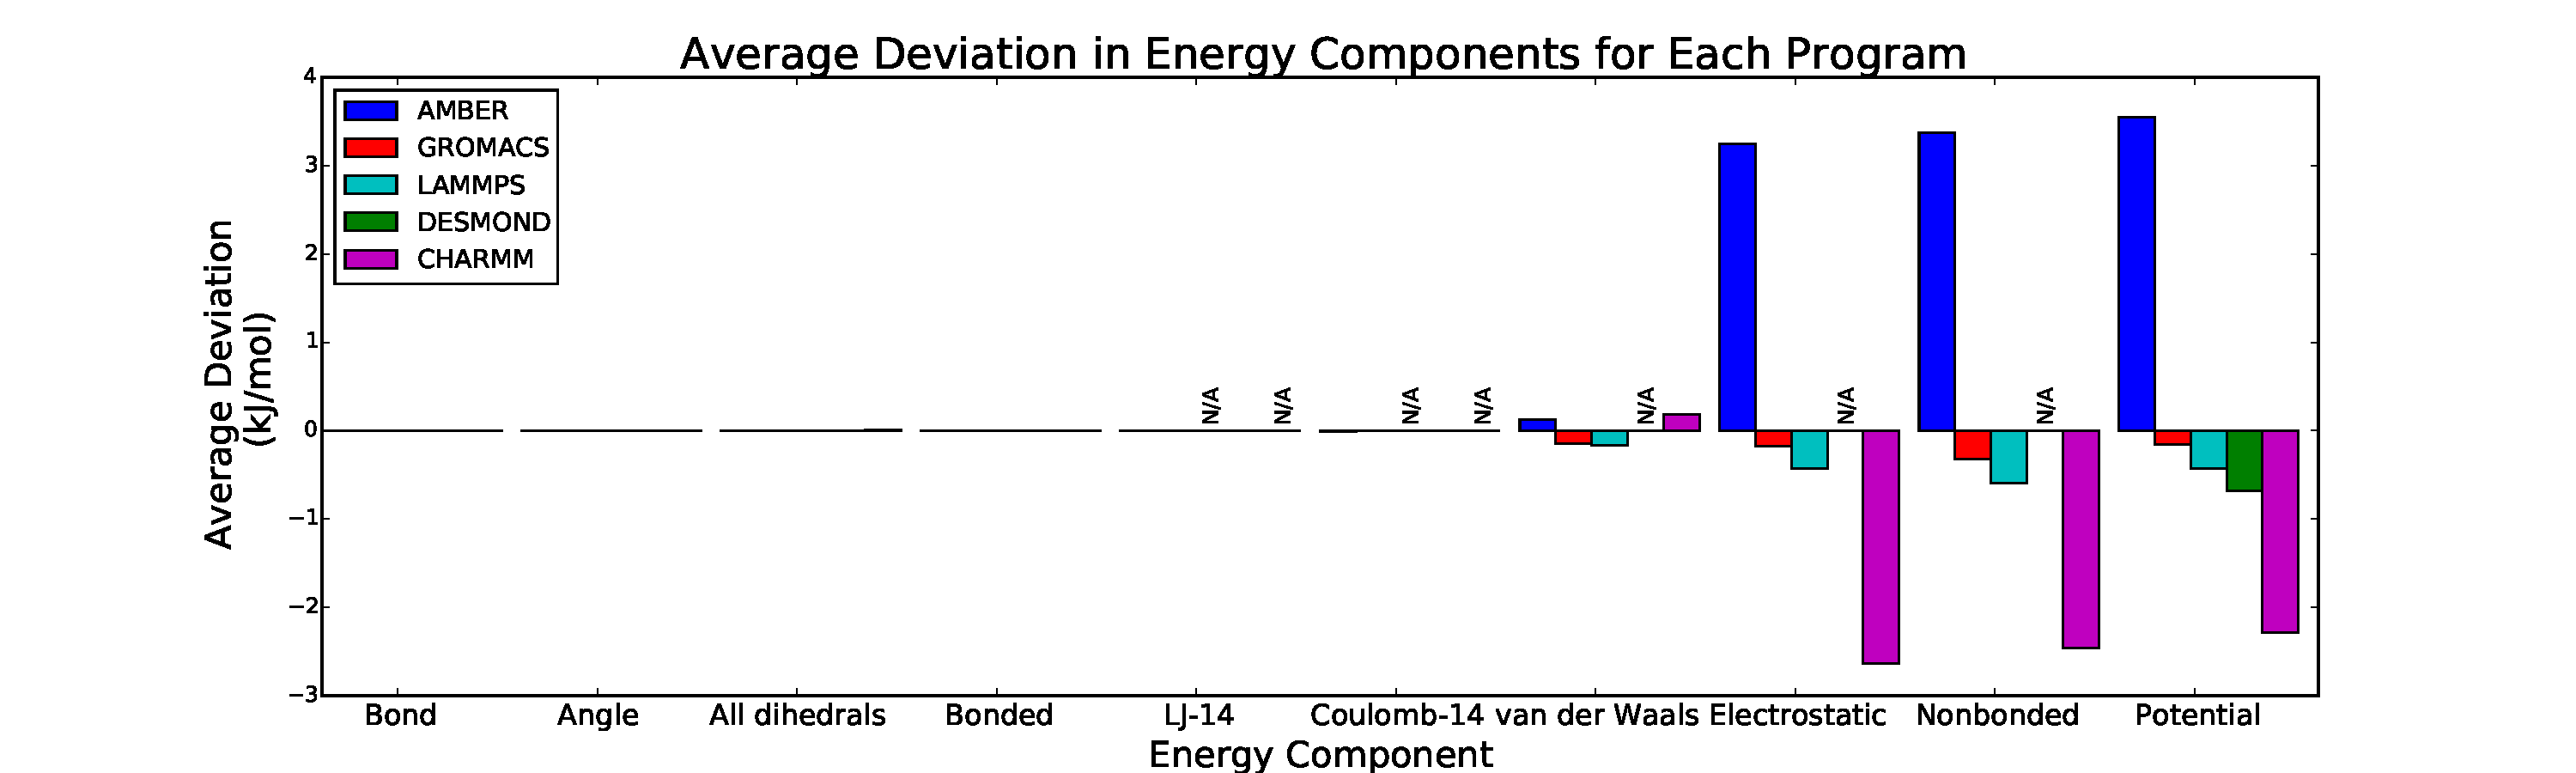
\includegraphics[width=\textwidth]{AverageIdealSettings.pdf} \\  
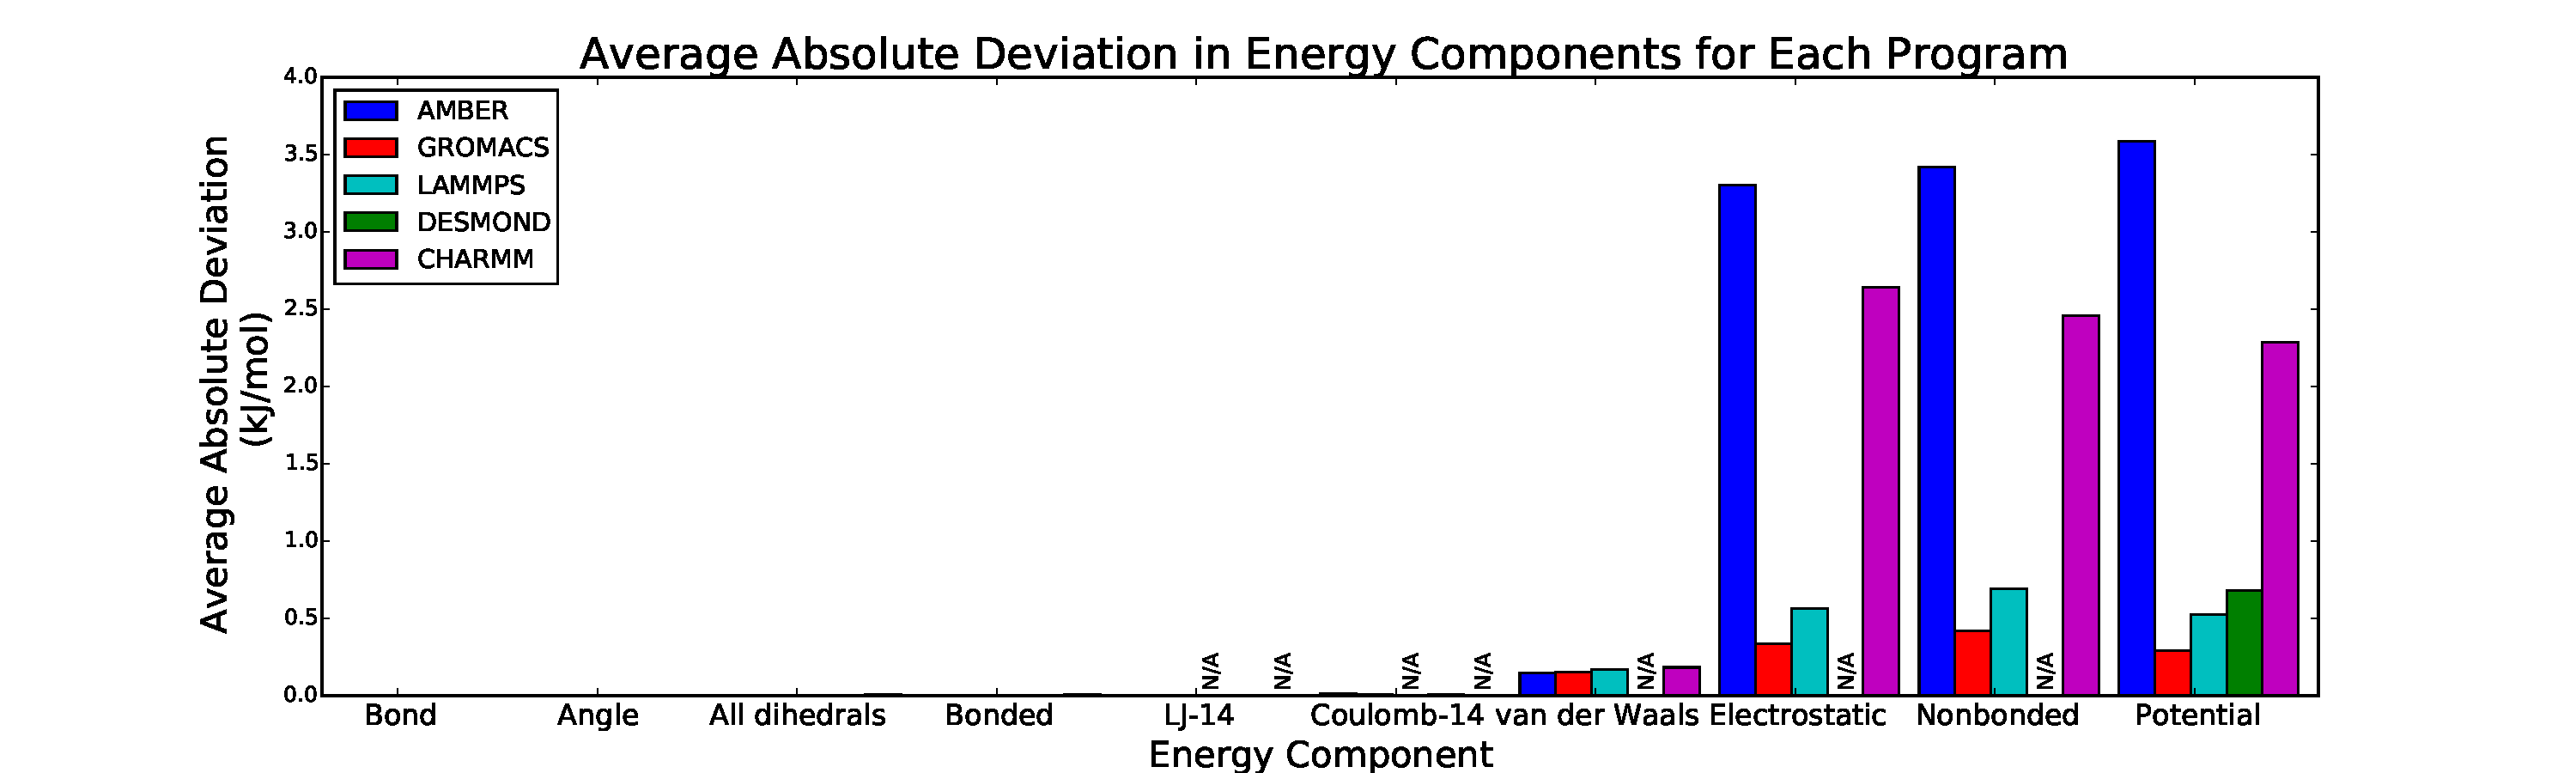
\includegraphics[width=\textwidth]{AverageAbsoluteIdealSettings.pdf} \\  
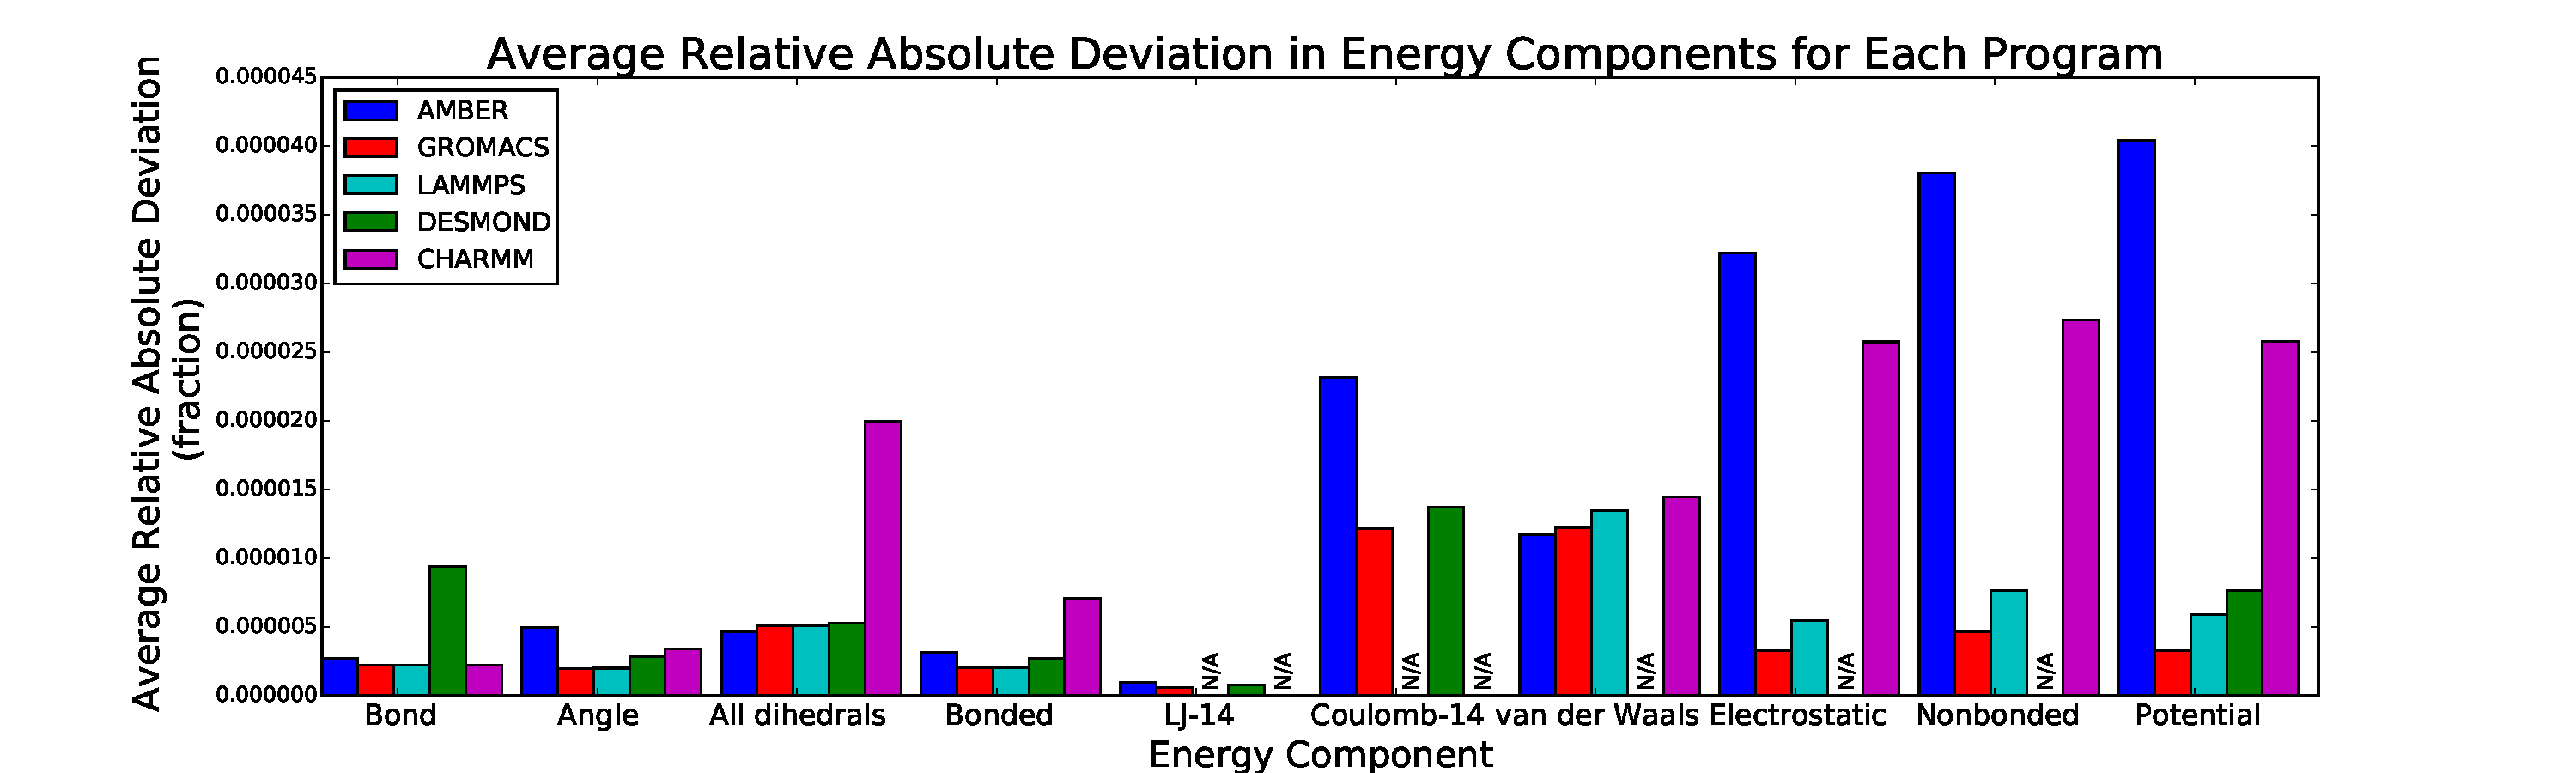
\includegraphics[width=\textwidth]{AverageRelativeAbsoluteIdealSettings.pdf}
\end{tabular}
\caption{Electrostatic energy interactions dominate the deviations
  between the programs both in absolute and relative error, though
  many components have measurable relative error. We compare the
  variation of 10 different energy terms between five different
  simulation programs (AMBER, GROMACS, LAMMPS, DESMOND, and CHARMM)
  for the 'ideal' choice of cutoff parameters. For each term, we plot
  the deviation of each program from the average over all programs
  (the program average), to avoid choosing a single arbitrary
  reference program. All statistics are averaged over the 22 SAMPL5
  host-guest molecules. We plot the average deviation (top), the
  absolute average deviation (middle), and relative absolute average
  deviation (top).
\label{fig:mainfig}}
\end{figure}
%DLM: Should the "average deviation" graph use some kind of log scale? Or a different scale for each component? Otherwise it seems sort of useless in that basically it just says that only the electrostatics is different by this metric. The "average absolute deviation" graph is similar except vdW starts showing up a hair more. On the other hand, maybe that's the point. I'm not sure - just a question, so use your judgment.
%MRS: added a bit more explanation.  Basically, I wanted to show that the electrostatic energy could go in both directions.

We next examine the nonbonded interactions. Coulomb 1-4 and van der
Waals 1-4 interactions are a good measure of whether the nonbonded
parameters are being copied correctly, as they generally are all
calculated with real space interactions and are shorter range than any
reasonable cutoff. Therefore, their comparison is not affected by
nonbonded simulation parameter choices such as treatment of long-range
electrostatics and represents the best test of Lennard-Jones
interactions and charges are properly copied from one set of files to
another.

We see that, like the bonded interactions, the 1-4 interactions, when
separated out from other interactions by the simulation program, are
in good agreement.  In all available cases, the van der Waals 1-4
interactions have relative absolute differences at least a factor of 2
better than even the bond and angle interactions, at about 1 part in
10$^{-7}$. LAMMPS and CHARMM do not calculate 1-4 interactions
independently, but some post-processing tricks involving subtracting
energies with different input parameters show that the CHARMM van der
Waals 1-4 energies have similar accuracy, in particular being
generally within output precision of AMBER.

The story from the Coulombic 1-4 interactions is more
complicated. Looking at the absolute difference, we see that the
difference of GROMACS and DESMOND from the program average is about
half of what the difference is from AMBER. In this case, the
difference in Coulombic 1-4 interactions between GROMACS and DESMOND
is actually less than 10\% of what the differences is between AMBER
and the other two programs is. Since the program average is the
average of the three programs, this means that essentially all the
deviation from the program average is because of AMBER's difference
from the other two programs.
%DLM: I can't follow that last sentence - too many "difference"/"differences". Is it saying that, if AMBER and the two other programs differ by X, then GROMACS and DESMOND differ by only 0.1*x, so (uh, I don't quite get it -- AMBER is the only weird one?).
%MRS: yes, tried to clarify. 
Since the LJ 1-4 parameters are shown to be in good agreement by the fact that the LJ-14 energies are in good agreement, 
%DLM "parameters"-> "energies"?
%MRS: clarified.
the difference must come from some other source.

After further analysis of the data, it became clear that the value of
Coulomb's constant $\frac{1}{4 \pi \epsilon_0}$, the constant of
proportionality $k$ in $U = k\frac{q_1q_2}{r}$ is the main cause of the
differences in the Coulomb 1-4 terms. In Table~\ref{tab:delfromnist},
we show the value of Coulomb's constant in a range of different
simulation programs compared to the NIST 2014 CODATA value.  We list
the AMBER number as``AmberTools''
%DLM: Isn't it "Antechamber" or "antechamber" now?
%MRS: fixed
because in AMBER, the constant is set by multiplying the charge by
$\sqrt{k}$ in the {\tt .prmtop} file, rather than set internally by
either {\tt sander} or {\tt PMEMD}, the AMBER molecular dynamics
engine.  Clearly, AmberTools, and to a lesser extent CHARMM, have
significant deviation from the best experimental value.  Personal
communication with Amber developers suggests that this difference may
come from mostly from in the 70's using Bohr's radius to calculate
Coulomb's constant assuming a value of 0.529167~\AA (versus an
improved value of 0.592177~\AA today, but there appears to be no clear
historical answer.  Of course, the more important question is, how
much this deviation affects the results?

\begin{table}
\caption{Values of Coulomb's constant currently used in molecular
  simulation programs compared to the value of 332.06371302(32)
  calculated from NIST 2014 CODATA.  Specific versions of the programs
  used are described in the text. Two versions of GROMACS are listed
  because SAMPL5 energies were originally generated with version
  5.0.4, but the value has been changed since then. Coulomb's constant
  was calculated as $k_e N_A e^2$, where $k_e$ is Coulomb's constant
  defined exactly in N m$^2$C$^{-2}$ (or J$\cdot$m$\cdot$C$^{-2}$),
  $N_a$ is Avogadro's number, and $e$ is the elementary charge from
  NIST 2014 CODATA, and then converted to kcal$\cdot$mol$^{-1}$ \AA
  e$^{-2}$. Non-SI units are used in this case because the number
  represents the value actually coded in the majority of programs.
  Uncertainties in $f$ were calculated using standard error
  propagation using NIST 2014 CODATA values at the correlation
  coefficient between $N_A$ and $e$ of -0.9985, also from NIST 2014
  CODATA. At less than 1000 standard deviations, however, errors due
  to Coulomb's constant are no longer the largest source of
  error.\label{tab:delfromnist}}
% Coulomb's constant in kcal/mol A / elementary charge^2 / nm 
% f = k_e * N_a * e^2 * 10^10/4184 
% f/ke = N_a * e^2 \approx  e^2 dNa + 2 Na e de 
% (f/ke)^2 = e^4 dNa^2 + 4 Na^2 e^2 de^2 + 4 Na e^3 C dNa de
% where C is the correlation coefficient.  
\begin{center}
\begin{tabular}{|ccc|}
\hline
Program & Value & $\sigma$ from NIST 2014 reference value \\
\hline
AmberTools &  332.0522173 & 51000 \\
GROMACS ($\leq$5.0) & 332.063693 & 89 \\
GROMACS ($>$5.1) & 332.0637138 & 3.3 \\ 
CHARMM & 332.054 & 43000 \\
LAMMPS & 332.06371 &  13 \\
DESMOND & 332.063762 & 220 \\
NAMD & 332.0636 & 510 \\
\hline
\end{tabular}
\end{center}
\end{table}

We tested the effect of changes in Coulomb's constant on the energy.
To add a more rigorous control, we looked at the RMS difference in
energy between AMBER energies and GROMACS energies evaluated with it's
5.0.4 Coulomb constant, and then with GROMACS recompiled with the
AmberTools Coulomb's constant.  Results are shown in
Table~\ref{table:coulchange}. We see that matching Coulomb's constant
removes 98.8\% of the difference in the Coulomb 1-4 term between the
two programs, 69.5\% of the total electrostatic energy difference, and
74.2\% of the total potential energy difference between the two
programs, strongly indicating that the lack of agreement of AMBER with
the other programs is almost entirely a result of mismatched Coulomb's constant.

\begin{table}
\caption{RMSD in kJ/mol of different energy components in GROMACS
  5.0.4 from AMBER energies as the GROMACS Coulomb's constant is
  varied. Averages are calculated over all 22 SAMPL5 host-guest
  systems.~\label{table:coulchange}}
\begin{center}
\begin{tabular}{|c|ccc|}
\hline
                          & Coulomb-14  & Electrostatic & Total Potential \\
\hline
GROMACS original constant &  0.00522    & 0.789         & 0.872  \\ 
AmberTools constant      &  0.000064   & 0.241         & 0.225 \\
Percent difference explained & 98.8\%   & 69.5\%        & 74.2\% \\  
\hline
\end{tabular}
\end{center}
\end{table}

The longer range nonbonded interactions are significantly harder to
get in good agreement between programs.  Validating the van der Waals
and Coulombic 1-4 interactions demonstrates that the Lennard-Jones
parameters and Coulombic charges are correctly created in the other
file formats.  In that sense, validating the conversion of file
formats can be done without comparing the long-range
interactions. However, if we are interested in comparing results of
molecular dynamics programs in realistic situations, we will need to
compare the entire potential energy, including these terms. 
%[NOTE: at
%  this point, we need to think about how important it is to answer
%  this question, and whether this document can answer it sufficiently]
%DLM: No comments here from me at this point - not sure. Seems fine without more on this to me.
%CTK: Also fine without

One complication is that different programs both calculate and print
out the different components of nonbonded interactions differently,
such as the direct space energy, the Fourier space energy, the Ewald
self term, and so forth.  Thus, it is often difficult to examine
anything except the total Lennard-Jones or total electrostatic
energy. This makes it hard to determine exactly the source of any
discrepancy between programs, and motivates our attempt to find
`ideal` simulation parameters to best make this comparison.

Discrepancies in the nonbonded energy terms are always much larger in
magnitude than discrepancies in the bonded interactions for any liquid
phase simulation, since there are many more intermolecular
interactions than intramolecular interactions.  It is therefore
instructive to look first at the average relative absolute deviations
from the program average. For GROMACS, AMBER, LAMMPS, and CHARMM, the
fractional difference in the van der Waals energy is approximately
$1\times 10^{-5}$, which is 2-5 times larger than the difference in
the bonded energy (DESMOND does not separate this energy out). GROMACS
and LAMMPS are generally closer to each other, usually within one part
in $10^6$, and CHARMM and AMBER are clustered together, though not as
closely as GROMACS and LAMMPS. Because of the close match of
Lennard-Jones 1-4 parameters, deviations in the total Lennard-Jones
energy are likely due to differences in the calculation of long range
interactions.

Differences from the program average in the total electrostatic energy
are smaller than errors in the total van der Waals energy for GROMACS
and LAMMPS, but are significantly larger for AMBER.  As seen above, a
large portion of the electrostatic deviation of AMBER from those two
programs is because of the inconsistent choice of Coulomb's constant.
Although CHARMM also has a relatively inaccurate Coulomb's constant,
the differences in the CHARMM potential energy are of opposite sign from AMBER, indicating a difference in the way the
electrostatic energy is calculated relative to the other programs.  
%[MRS: Address.
%  this is the one place I'm a little worried about whether I am
%  running a simulation correctly, and will follow up with CHARMM
%  people] 
%CTK: The opposite sign also seems peculiar to me. Would be good to pin
%down.
%MRS: haven't been able to track it down by myself, will need to ASK charmm people)
For AMBER, about 70\% of this deviation is due to 
Coulomb's constant choice, leaving significantly less of the deviation
from other programs due to other choices in nonbonded simulation
parameters. An adjustment in CHARMM's Coulomb's constant would
actually make the energy further from the other three programs.
However, it is important to notice that the fractional difference is
still on the order of $2.5 \times 10^{-5}$, likely too small to matter
for most quantities of interest over long simulations.

The deviations in the program average of the total potential energy is
dominated by the differences in the nonbonded terms, since those are
so much larger than differences in the bonded energy.  For CHARMM and
AMBER, differences in the electrostatic nonbonded energy
dominates. DESMOND total potential energies differences from the
program average are almost the same as GROMACS and LAMMPS, indicating
that since the bonded interactions match the two programs well, the
nonbonded also must agree relatively well.

\begin{figure}[h]
\begin{tabular}{c}
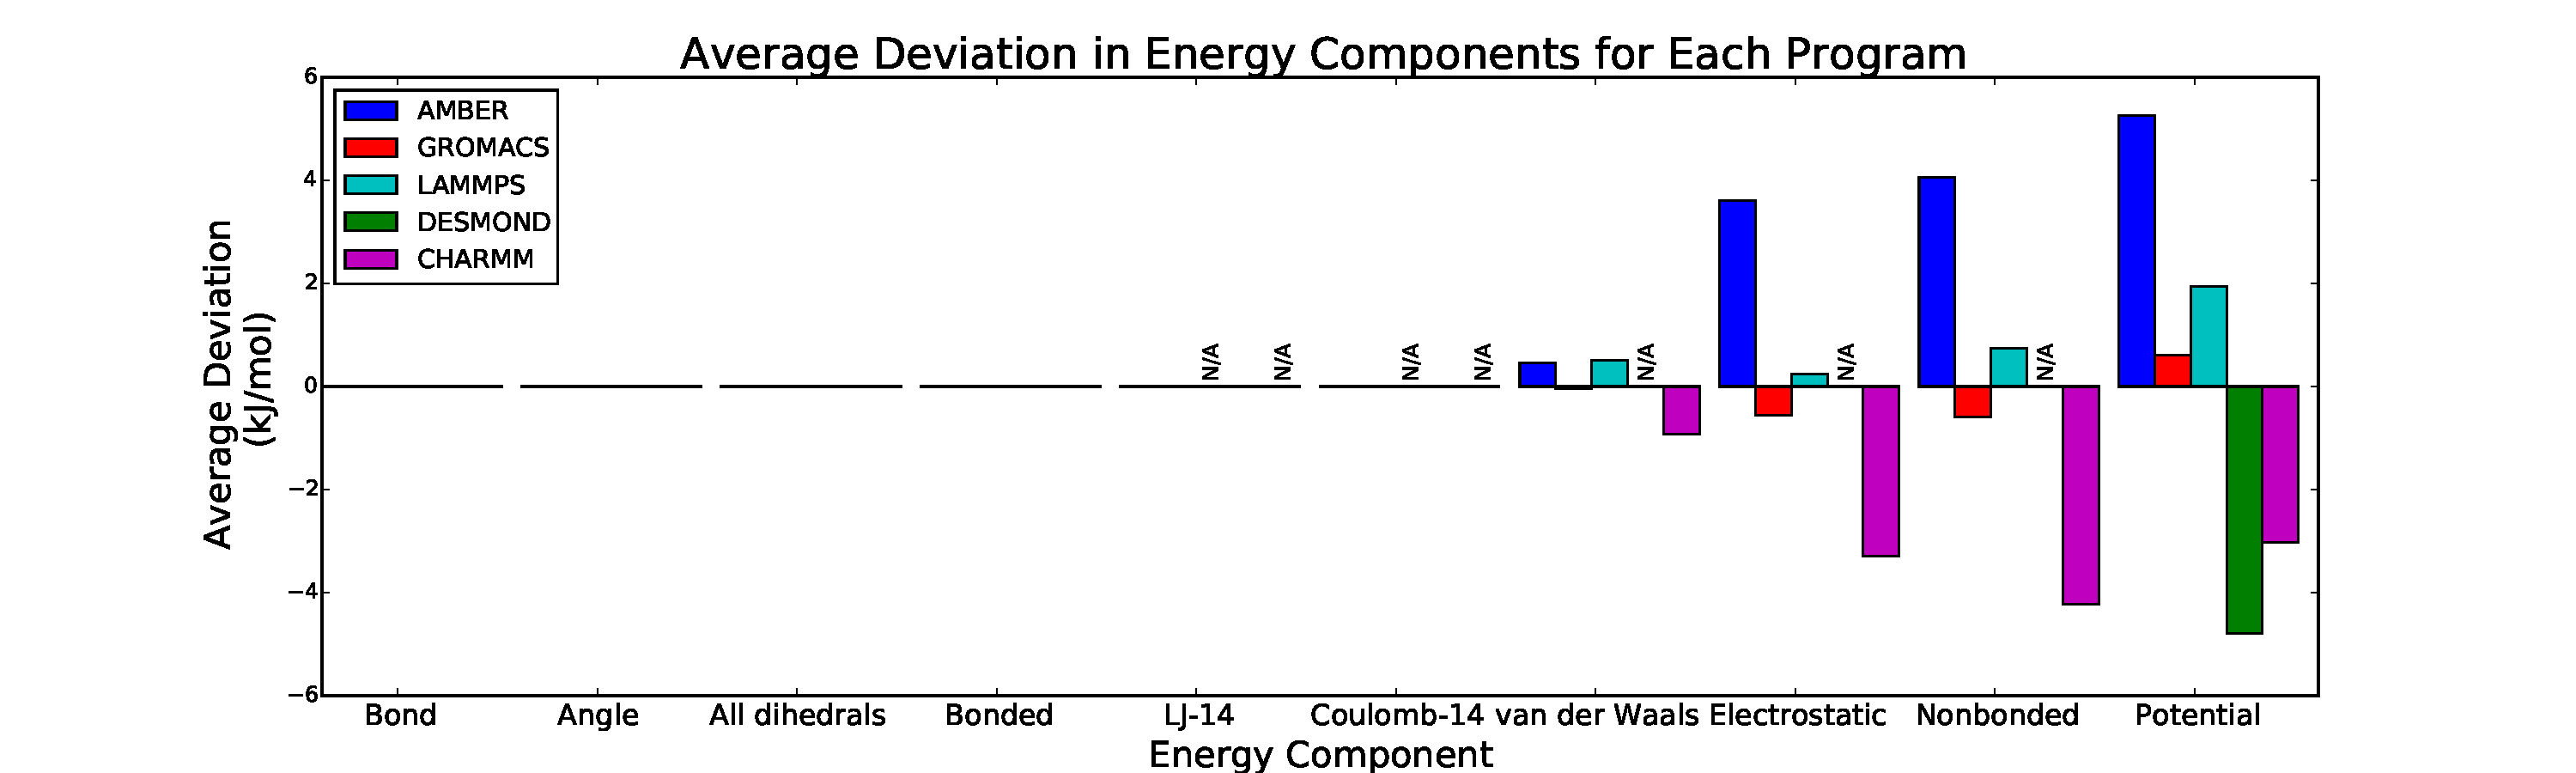
\includegraphics[width=\textwidth]{AverageDefaultSettings.pdf} \\  
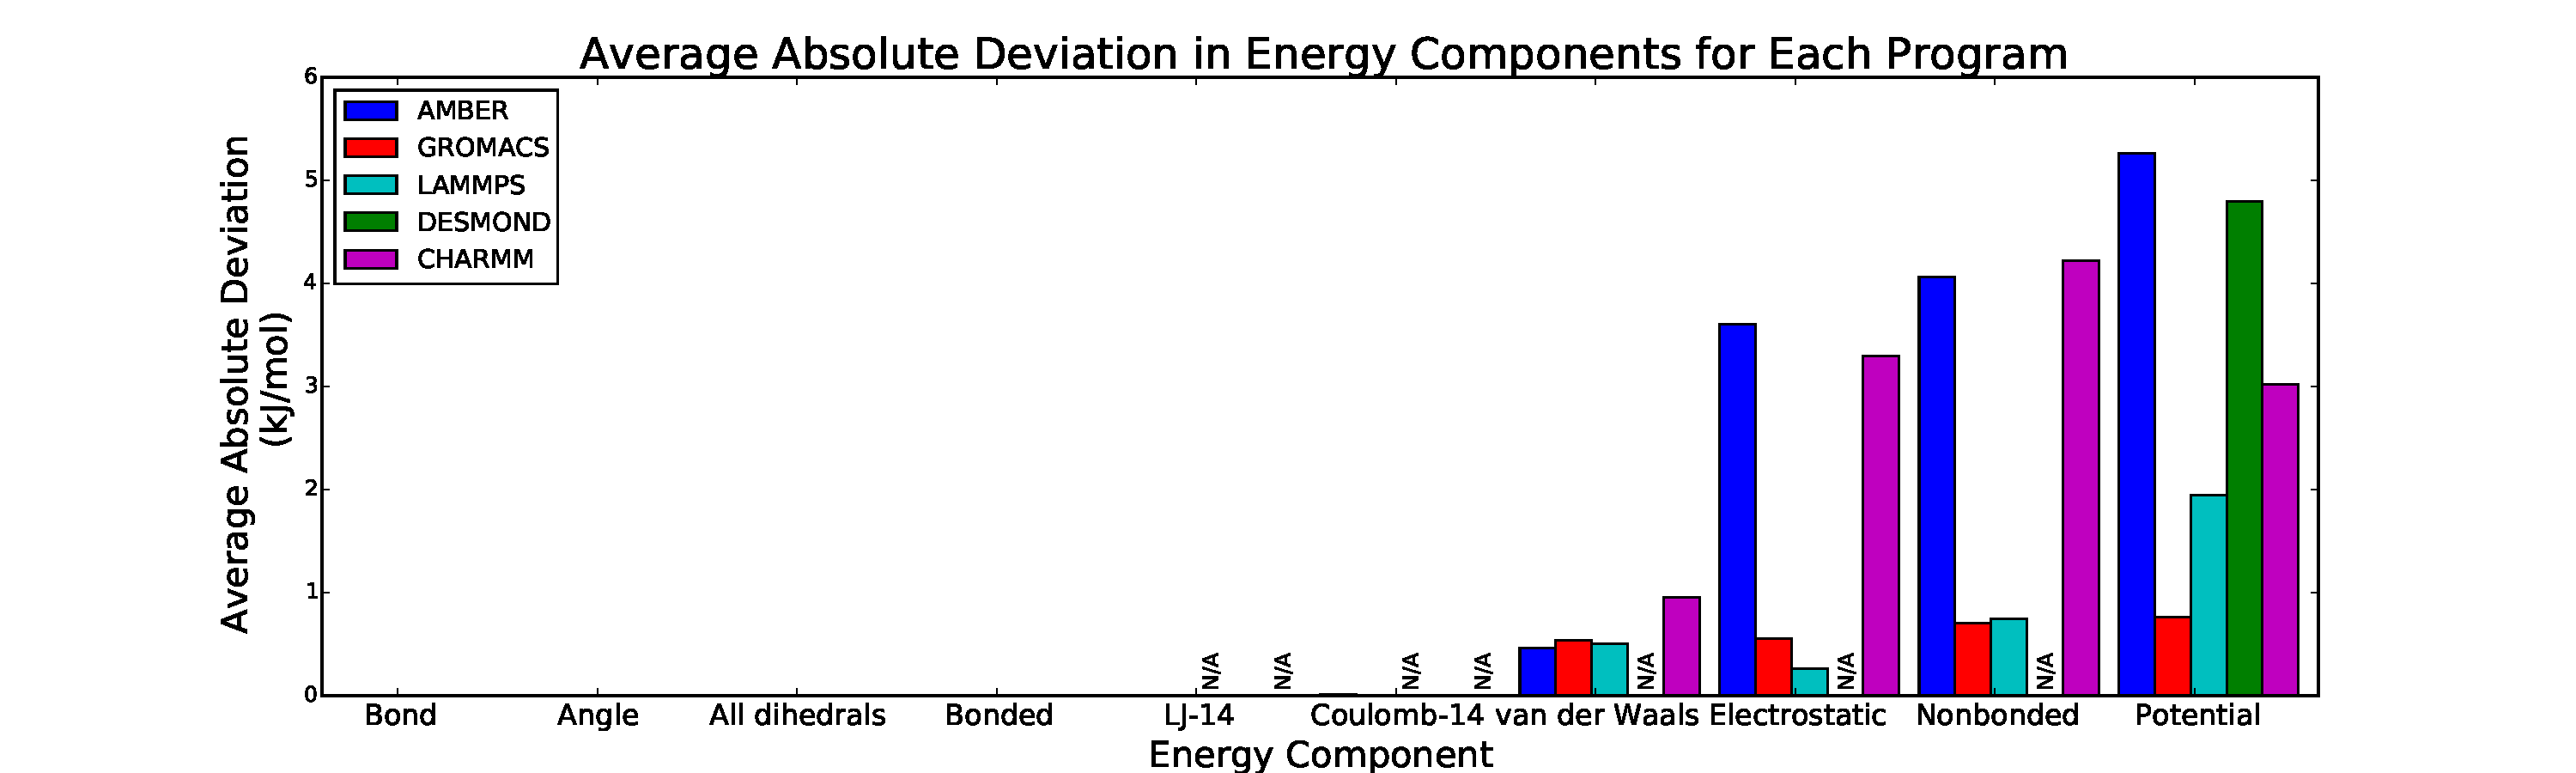
\includegraphics[width=\textwidth]{AverageAbsoluteDefaultSettings.pdf} \\  
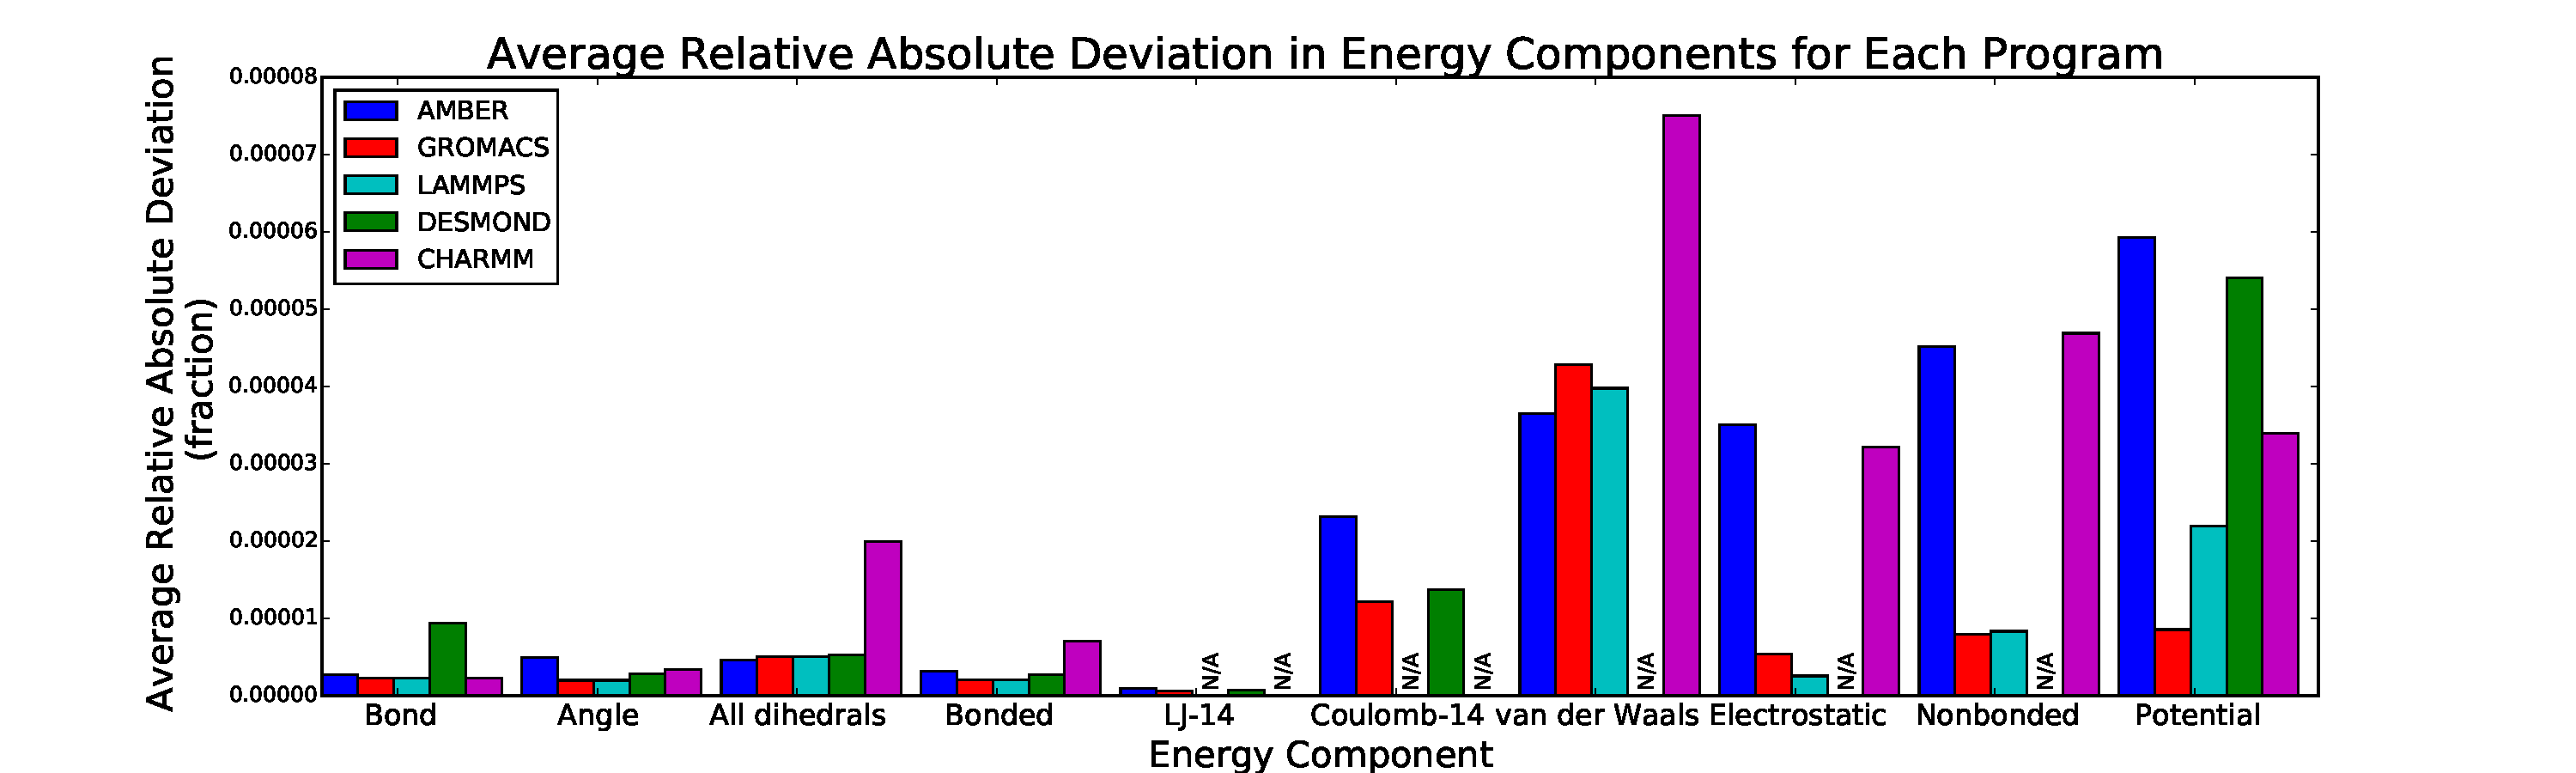
\includegraphics[width=\textwidth]{AverageRelativeAbsoluteDefaultSettings.pdf}
\end{tabular}
\caption{We compare the variation of 10 different energy terms between
  five different simulation programs (AMBER, GROMACS, LAMMPS, DESMOND,
  and CHARMM) for the 'default' choice of cutoff parameters (described
  in table). As above, for each term, we plot the deviation of each
  program from the average of all programs, to avoid choosing a single
  arbitrary reference program. All statistics are averaged over 22
  molecules. We plot the average deviation (top), the absolute average
  deviation (middle), and relative absolute average deviation
  (top). Nonbonded potential parameter deviations are approximately a
  factor of 2 larger than using the 'ideal' parameters.
\label{fig:defaultfig}}
\end{figure}
%CTK: This figure is never cited within the text as far as I can tell...

We also are interested in the deviations of energies as a function of
the number of coordinates used in the output file. The results of the
comparison between AMBER (full precision input) and GROMACS (reduced
precision output) are shown in Fig.~\ref{fig:precision}.  We choose
only to show GROMACS as the other programs show similar behavior. We
plot the $-\log_{10}$ of the average relative absolute difference
between the GROMACS energy and the AMBER energy as a function of the
number of decimal places in the output GROMACS coordinates from 8
digits after the decimal place (measured in nanometers) down to 4
after the decimal place, what one would obtain from a file downloaded
from the PDB.  

We see that the total energy loses approximately 0.75-1 digits of
relative precision in the energy for each digit of precision of
coordinate lost. Since the van der Waals and electrostatic nonbonded
energies contribute the majority of the potential energy, their loss
of precision mirrors the overall loss of precision. Interestingly, the
bonded and both 1-4 terms are less sensitive to changes in coordinate
precision, not losing much precision until getting down to 5 or fewer
digits after the decimal point. Bond and angle terms individually lose
precision, but the dihedral energy dominates the total bonded energy.
Both Lennard-Jones and electrostatic nonbonded energies fall off
similarly in precision, so large errors in the repulsive $r^{-12}$
interactions do not seem to be larger than changes in the Coulombic
$r^{-1}$ terms as the coordinates become more approximate.

Overall, losing just a few digits of precision completely washes out
any other source of error observed in this study, demonstrating the
importance of matching the coordinates to high precision in order to
validate the rest of the conversion.

\begin{figure}[h]
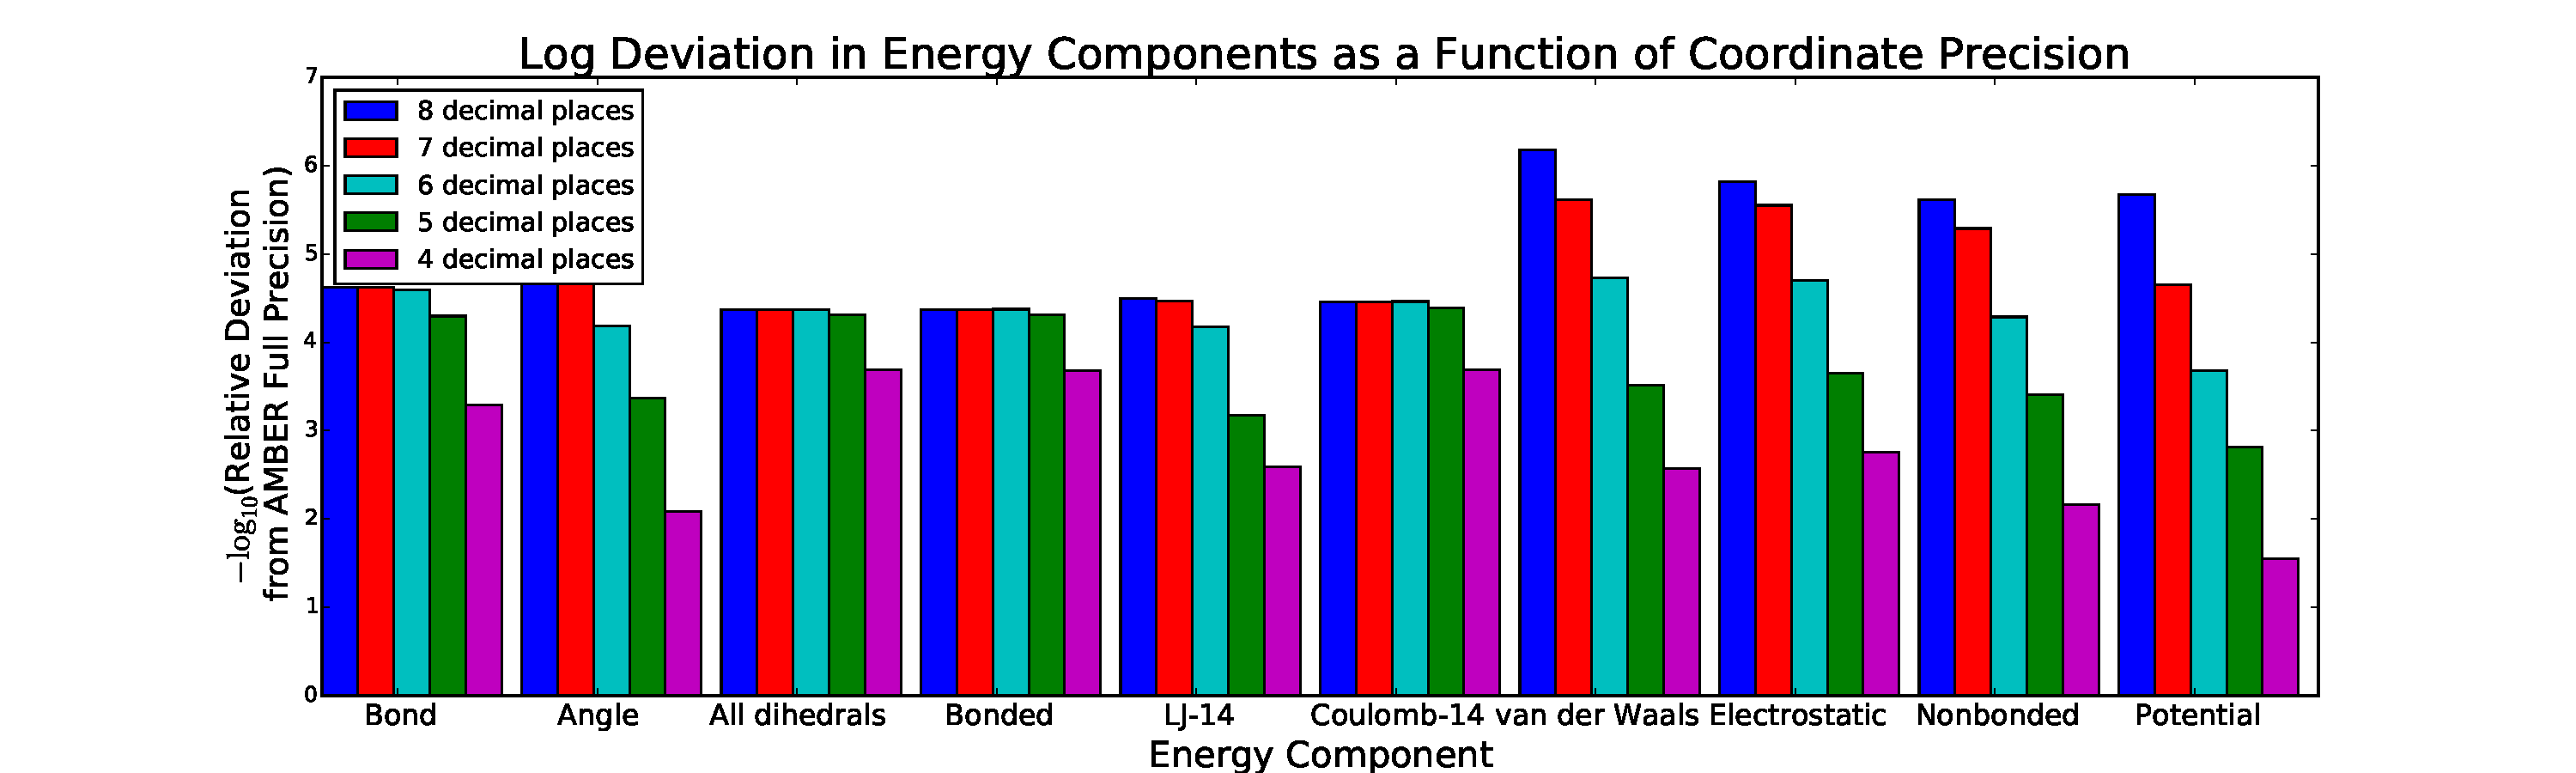
\includegraphics[width=\textwidth]{precisioncomparison.pdf}   
\caption{Matches in energy between converted files become rapidly
  worse as the number of digits of precision in the converted files
  decreases. We plot $-\log_{10}$ of the average relative absolute
  value in each energy term between AMBER and GROMACS, with fixed
  input coordinate precision, and variable output precision with the
  number of decimal places in the coordinates in nanometers, varying
  from 8 down to 4, the precision of a standard PDB file.
\label{fig:precision}}
\end{figure}

We are also interested in how much changing the precision of the
binaries affects energy comparisons.  We focus on the comparison
between single and double precision GROMACS, as it is specifically
designed to be compiled in either single and double precision, though
the single precision is the default version most simulations are run
with. In Table~\ref{fig:singlevdouble}, we compare the RMS differences
averaged over all 22 compounds between the two GROMACS binaries, AMBER
and single precision GROMACS, and AMBER and double precision GROMACS.
This comparison allows us to see both the magnitude of the difference
due to changes in binary precision, and how much this differences
affects the comparison to, for example, AMBER.

We see that the differences between single and double precision show
in Table~\ref{fig:singlevdouble} for bonded terms is 2-8 times larger
than the difference between AMBER and double precision GROMACS, and is
usually the dominant contribution to the difference between AMBER and
single precision GROMACS.  Differences between the precisions for
LJ-14 is about equal to differences between either precision and
AMBER.  Differences between precisions for Coulomb-14 terms is as low
as the difference between LJ-14, which is of course much less than the
GROMACS to AMBER difference, because of the previously described
difference in Coulomb constant. The differences in precision for the
total van der Waals is an order of magnitude lower than the difference
between AMBER and either GROMACS precision caused by differences in
calculating the long-range nonbonded terms.  However, single to double
precision change results in significant difference in the overall
electrostatic term, as large as the magnitude between GROMACS and
AMBER.  Because the total van der Waals energy changes relatively
little between precisions, it is likely that the short-range
electrostatics (which are functions only of the distance) are also
relatively accurate, and it is the Ewald summation part that changes
upon changes in binary precision.
%DLM: I must not be able to read the graph, as this sounds like you're saying almost the opposite of what I'd conclude from reading the graph. To me, I'm looking for where the -log( relative deviation) falls off fastest, so it looks to me like vdW, nonbonded, potential, and angle (i.e. I'm looking for where the "4 decimal places" bars are lowest relative to the "8 decimal places" bars...). But here it sounds like you're saying that the biggest changes come from Coulomb-14 is the worst offender, and I don't get that at all... How am I supposed to see that from the graph?
%DLM: I'm putting this here not so that you explain it to me, but so that you understand why I'm confused and revamp the discussion of this in the text and the figure caption to make more clear what I'm supposed to see and how I'm supposed to understand it. :) 
%CTK: @ DLM, not sure if this is the point of confusion but the above
%paragraph is talking about the table comparing single vs. double prec,
% not the figure comparing coordinate precisions.
%MRS: see CTK - this is the table, not the graph.

\begin{table}
\begin{tabular}{|c|ccc|}
\hline
E term & RMS($E_{single} - E_{double}$) &  RMS($E_{amber} - E_{single}$) &  RMS($E_{amber} - E_{double}$) \\
           Bond &   0.000066 &   0.000068 &   0.000008\\
          Angle &   0.000044 &   0.000043 &   0.000007\\
  All dihedrals &   0.000015 &   0.000031 &   0.000018\\
         Bonded &   0.000081 &   0.000086 &   0.000011\\
          LJ-14 &   0.000013 &   0.000020 &   0.000025\\
     Coulomb-14 &   0.000007 &   0.001250 &   0.001251\\
  van der Waals &   0.001894 &   0.021756 &   0.023116\\
  Electrostatic &   0.218874 &   0.403839 &   0.189265\\
      Nonbonded &   0.217209 &   0.422827 &   0.209207\\
      Potential &   0.217134 &   0.422781 &   0.209214\\
\hline
\end{tabular}
\caption{\label{fig:singlevdouble}Differences between double and
  single GROMACS energy evaluations are of similar magnitude to the
  differences between AMBER and GROMACS, but are dominated by
  differences in the long-range electrostatics. All energies in kJ/mol.}
\end{table}

We are also interested in how much of the differences between programs
vary with the configurations of each molecule. For example, if we were
to take different configurations of the same molecule, would we get
similar deviations from the program average for all of the molecules?
We ask this question by taking the 12 octa-acid hosts, and generating
20 configurations as described in the Methods section using NVT
molecular dynamics. The average over these 20 configurations is a rough approximation to the ensemble average energy of the
system.

We then compare the RMSD from the program average $\sigma_{config}$,
averaged over all $12 \times 20 = 240$ configurations, and the RMSD of
the average energy of all configurations of the same molecule from the
program average over the 12 host-guest systems$~\sigma_{molecule}$. If
the variation from program to program is independent of configuration,
and only dependent on the differences between molecules, then we would
expect that the two different RMSDs would be roughly equal, meaning
there is low conformation dependent variation.  If instead the
variation is independent of the specific molecule, and depends on
interactions from random atoms, independent of the molecule, then the
RMSD from the configurationally averaged deviations from program
averages ($\sigma_{molecule}$ would be significantly smaller
(approximately $\sqrt{1/20} \approx 22$\% of the value
$\sigma_{conformation}$ value.
% Note that the RMSD of the conformationally averaged values
%must necessarily be lower than the RMSD over all configurations and
%molecules. 
The extent to which $\sigma_{molecule}$ is smaller than
$\sigma_{config}$ shows how much of the variation is inherent to the
molecules, and how much is only dependent on the configurations.
%DLM: This is hard to follow.
%MRS: Attempted to clear up, probably not yet great.

We can quantify this difference in the source of variation by
calculating the fraction of the total variation due to conformational
variability, calculated as
$\frac{\sigma^2_{config}-\sigma^2_{molecule}}{\sigma^2_{molecule}}$,
for each energy term. If this quantity is low, then variation is
mostly due to differences between molecules, not configurations.  If
it is near one, then variation between programs is mostly due to
changes in conformation.

We can observe the results in Figure~\ref{fig:confvariability}. At one
extreme are the bond energies, which have only about 8\% of the total
variation between programs due to configurational variation, near the
minimum of 1/20 $\approx$ 5\%. Most of the differences are due to
differences between the molecular bond terms, but not the specific
conformation.  Similarly, the variations in van der Waals 1-4
interactions are mostly due to differences between molecules.

At the other extreme are the Coulomb 1-4 terms, where almost 100\% of
the variation is due to conformational variation: after averaging the
differences over molecules, there is very little variation left due to
conformational changes. It is not entirely clear why Coulomb 1-4 and
van der Waals 1-4 are so different in patterns, given that they are
both primarily determined by the locations of the same set of 1-4 atoms.
Similarly, almost 100\% of the variability in the total van der Waals
energy is due to conformational variability.  Variation in angle
energies from the program average again likely relatively dependent on
configuration (around 80\%). 
%MRS: ADDRESS [NOTE: I don't entirely understand the
%  differences between LJ-14 and Coulomb-14.  I need to think about it
%  a bit more.]
%MRS2: haven't been able to think about this well yet.
Total electrostatic variation is one of the few energy components
where the fraction of conformational variation depends significantly
on the programs.  For AMBER, it is not very dependent on
configuration; for other programs, it is much more dependent on
configuration. This is likely because of differences in Coulomb's
constant and in the treatment of long-range electrostatic energies,
%DLM: I don't understand how the AMBER choice of Coulomb constant could make the results more dependent on configuration. If this is the case you have to explain the logic here more.
%MRS: The next section is the logic, tried to tie it together better.
Coulomb's constant changes can make such a difference because the
long-range energies are much less dependent on individual molecular
distances, instead being dependent on the average distribution of
charge within the system, which does not change significantly for a
host-guest system over time, and which will scale with the changes in
Coulomb' constant.  On the other hand, the Coulomb 1-4 interactions
are dominated by the variability of which atoms are closest to each
other at any given time, which is larger than the Coulomb constant
differences.

The analysis in the variation of the total potential energy conclusion
illustrates again that the dominant reasons that the molecular
simulations differ are the evaluation of long-range interactions,
especially the electrostatics, and the choice of the Coulomb
constant. We find that the total variation of the potential energy,
like total potential energy itself, depends almost entirely on the
nonbonded terms.  Since the van der Waals variation between programs
is almost entirely conformation dependent, with very little deviation
in programs between the ensemble average estimate for each molecule,
the conformational dependence of the total energy is essentially
determined by the conformational dependence of the electrostatic
energy. The bonded terms are essentially irrelevant.


\begin{figure}[h]
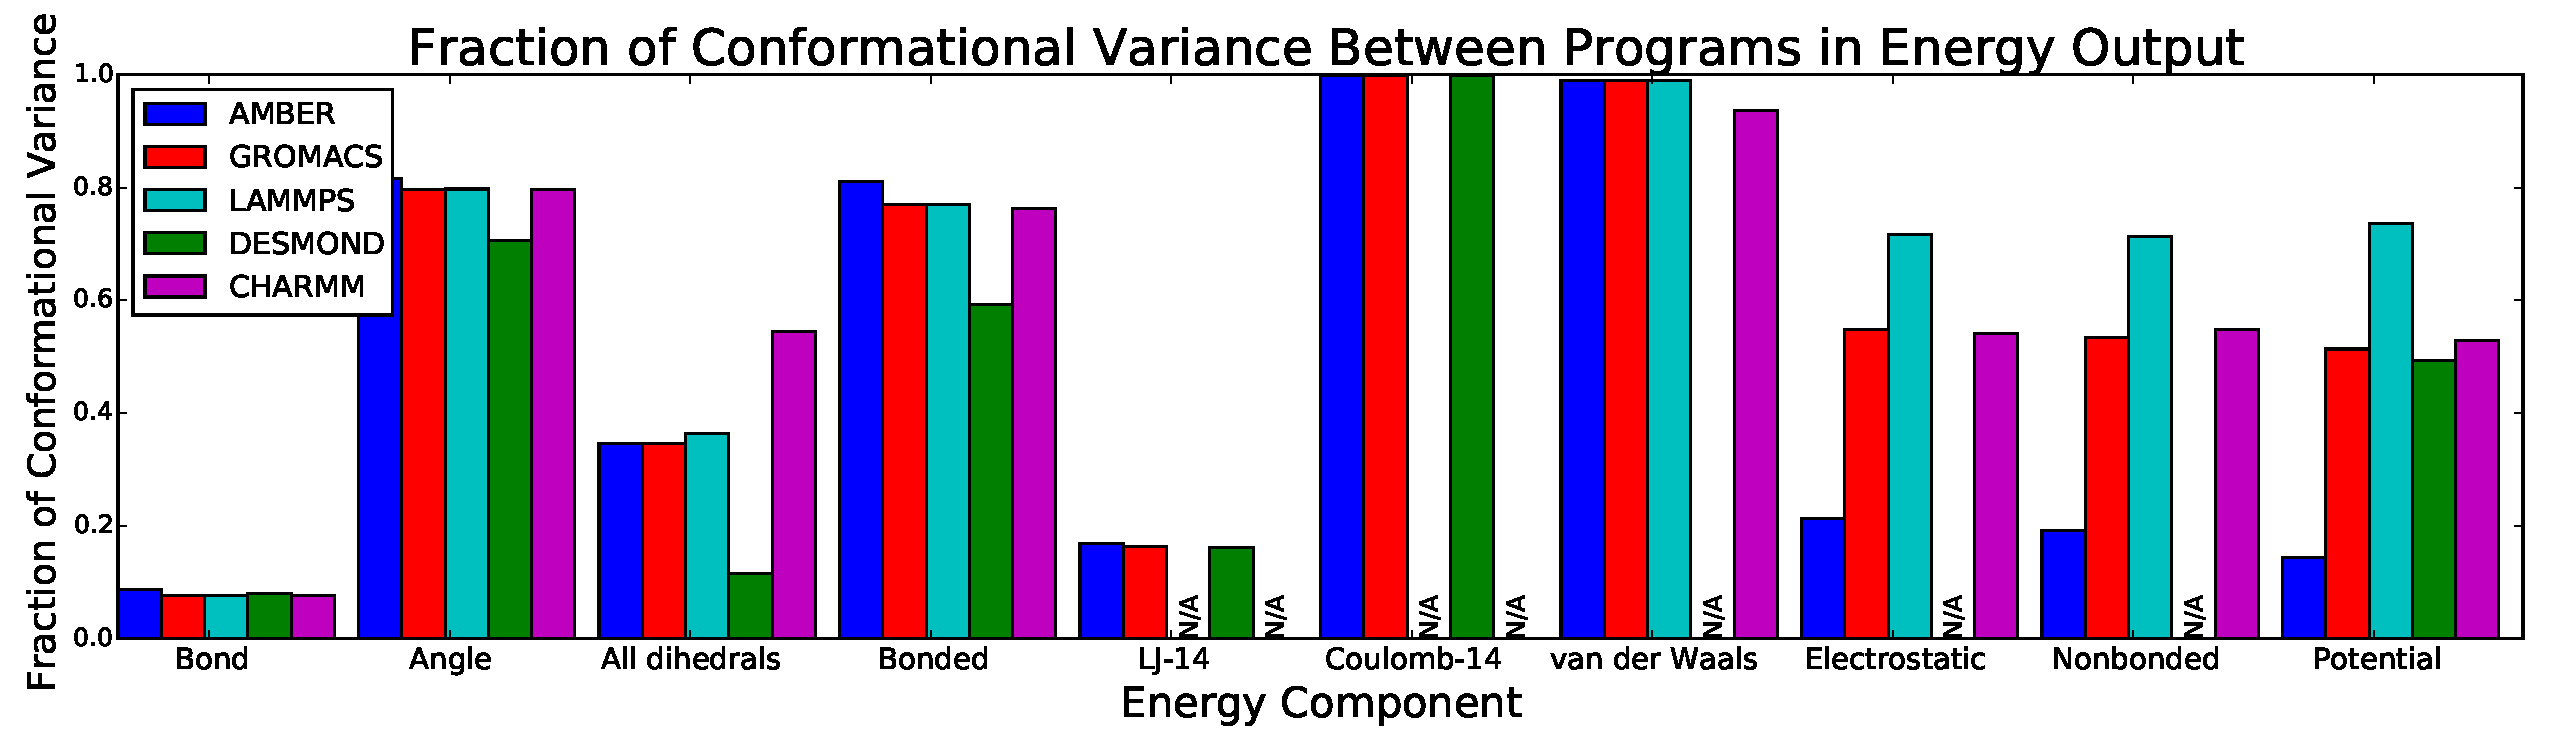
\includegraphics[width=\textwidth]{fractionofvariation.pdf}   
\caption{Fraction of variation from the program average due to
  conformational variability instead of molecular variability,
  calculated as
  $\frac{\sigma^2_{config}-\sigma^2_{molecule}}{\sigma^2_{molecule}}$,
  where $\sigma_{config}$ and $\sigma_{molecule}$ are standard
  deviations from the program energy over all configurations and over
  molecule averages, respectively.
\label{fig:confvariability}}
\end{figure}
%DLM: In the interests of making figures intelligible on their own, this one needs more details, as I don't understand "fraction of variation... due to..." in this one. Is it saying that of the total variation in bond energy (of what?) how much of it is due to the choice of conformation used? 
%MRS: tried to address more.

\section*{Discussion}

\subsection*{Issues in file conversion}
Creating true all-to-all functionality is particularly
difficult. There are a number of one-to-one conversion utilities and
scripts: for example, ACPYPE~\cite{sousa_da_silva_acpype_2012},
CHAMBER~\citep{crowley_chamber:_2009}, and {\tt amber2lmp}.  We have
developed InterMol and ParmEd as (at least in part) all-to-all
converters, though neither yet manages to interact with all programs.
A truly all-to-all converter (rather than the nearly all-to-all
process set up in this study) would substantially simplify the current
painstaking process of molecular simulation conversion.

There are a number of differences between programs not immediately
obvious that nonetheless need to be carefully matched for the same
system to be represented in both programs.  For example, GROMACS
builds lists of 1-4 interactions based on the bond topology: if three
bonds connect two atoms, they are 1-4 interactions. However, AMBER
uses the presence of dihedrals to define 1-4 interactions. A dihedral
with zero energy in GROMACS is essentially redundant and can be
eliminated without affecting the energy, but creates 1-4 interactions
in AMBER.  Additionally, the same interaction in different programs
may have different names, functional formats. This can either be
handled by hard-coded conversions (ParmEd) or converting all
interactiosn to an from a canonical form (InterMol).  The first has
the advantage of readabilty, whereas the second is more general.  It
is not yet clear what the optimal strategy should be.

 One of the most challenging problems in conversion of molecular
 simulation files is handling the different units in each simulation
 engine. Both InterMol and ParmEd address this problem by
 automatically convert units between simulation input files, removing
 the needs for manual unit conversion. This is handled by creating
 data types that carry units with them, making conversion much
 simpler.  Without such unit-carrying data types, doing anything other
 than one-to-one conversion becomes signficantly harder.

In order to aid further analysis of the energies, all energy output
and summarized analysis presented here in this paper is provided in
the 'analysis.tgz' directory in the supporting information, as
described in the 'README.txt' supporting information file.

\subsection*{Issues in matching energies}

It is difficult to say what the ``right'' energy is for a system, as
there are several different reasonable choices for implementation of
long-range interactions. For a sufficiently large box, one could
simply extend out the cutoffs, treating an increasingly larger amount
of the system using straightforward direct space interactions.
However, these systems, at 4.0 nm across, are not large enough to take
the direct-space electrostatic treatment out far enough for the
different programs to completely converge together.  This remains a
key weakness of the study, making it difficult to decide on a single
reference energy to compare the simulations. This resulted in our
choice to examine deviations from the program average, rather than
attempt to determine the correct energy. 

%[NOTE: I could build a really big box of water and see which
%  simulation approach converged best to really long short range
%  cutoffs, and rank the approaches that way.]
%DLM: I think the language here and above needs to be clearer. It sounds like you're saying you're interested in comparing energies for large systems with long cutoffs and no lattice-sum electrostatics (which you're calling "short-range interactions") to energies for large systems with short cutoffs and lattice-sum electrostatics. Is that right? If so maybe say so specifically. Otherwise there is some ambiguity about what you mean by "short-range interactions", since I don't normally think of, say, Coulomb interactions at a distance of 2 nm as "short range" in a simulation context. :) 
%MRS: tried to clarify.

\section*{Conclusions}
The results presented here show that the simulation input files are
properly converted by the very strong agreement, essentially within
single precision calculations, for all bonded terms, Lennard-Jones 1-4
terms and (with one caveat outlined below) Coulomb 1-4 interations. 

We believe that this study represents the largest automated comparison
between different programs that has been performed so far, a process
only possible because of the automated conversion. The pipeline
described in this program, properly scaled up for diverse ranges of
systems, could be useful for a range of comparison studies that
require the precise comparsison across multiple simulation engines, or
in modeling pipelines that require one simulation program for part of
the pipeline, and another simulation engine for a different part.

The results also strongly suggest that all molecular simulation
programs should choose a sufficiently consistent value for Coulomb's
constant. A value off of experiment by 0.01 from a value of 332.06371
(one part in 10$^{-5}$) is simply not accurate enough to allow
simulations to agree.  The results presented here suggest that once
the deviation is below 0.0001, any additional error contributes less
than other sources of error, so a value of 332.06371$\pm$0.00005
should reduce this sort of discrepancy below the level of differences
created by other programs.  This level of agreement is present in all
current programs with the exception of CHARMM and AMBER, with GROMACS,
at the edge of that range, recently improving the precision by a
factor of 4 in the 5.1 release.

Other than the difference in Coulomb's law, most programs agree quite
well, likely enough for most practical purposes as most thermodynamic
quantities cannot be measured that accurately.  All conversions were
performed accurately and the model parameter conversion was validated
to high precision. Only the long-range interactions deviated by
moderate amounts between programs, especially the electrostatic
Fourier-space interactions.  Even those differences are unlikely to
affect most thermodynamics studies.

\begin{acknowledgements}
The authors would like to thank Frank Pickard (NIH) for sample CHARMM
inputs and discussion about evaluation of CHARMM energies, Justin
Lemkul (U. Maryland) for advice on CHARMM functional form, and Chris
Lee (U. Va., UCSD), Alex Yang (U. Va.), Michael Zhu (U. Va.), Hari
Devanathan (U. Va.), and Jacob Rosenthal (U. Va.)  for initial work on
InterMol. DLM thanks NSF (CHE 1352608) for financial support.
\end{acknowledgements}

% BibTeX users please use one of
\bibliographystyle{spjcamd}
%\bibliographystyle{spbasic}      % basic style, author-year citations
%\bibliographystyle{spmpsci}      % mathematics and physical sciences
%\bibliographystyle{spphys}       % APS-like style for physics
\bibliography{JCAMD_citations,Zotero}   % name your BibTeX data base

% Non-BibTeX users please use
%\begin{thebibliography}{}
%
% and use \bibitem to create references. Consult the Instructions
% for authors for reference list style.
%
%\bibitem{RefJ}
% Format for Journal Reference
%Author, Article title, Journal, Volume, page numbers (year)
% Format for books
%\bibitem{RefB}
%Author, Book title, page numbers. Publisher, place (year)
% etc
%\end{thebibliography}

\end{document}
% end of file template.tex


% LocalWords:  tex SVJour EPS cucurbit uril octa der waals vdW SAMPL PACS MSC
% LocalWords:  nominalizations CB OA Moghaddam Muddana Gallicchio Jayachandran
% LocalWords:  Lyubartsev Escobedo Desgranges solute Christoph Swails Jian TN
% LocalWords:  Gilson Zhong Skaggs San CA VA GROMACS LAMMPS CHARMM ParmEd NVE
% LocalWords:  InterMol Coulomb's deconvolute microcanonical NVT limitating NJ
% LocalWords:  Lennard SPME kJ acepype intercoversion py API nonbonded CBClip
% LocalWords:  OAH OAMe MOE sulfonic carboxylic protonation pKas RESP HF Joung
% LocalWords:  atm solutes SI odinger dms cms charmm lite RHEL gcc DLM JMS NpT
% LocalWords:  PPPM CC lj Langevin timestep nonbondeds html nx ny nz doesn Rtol
% LocalWords:  tol coul pre lammps CCCCCCCCCC NIST CODATA Avogadro's ke dNa Na
% LocalWords:  de NAMD Pickard NIH Justin Lemkul Zhu Hari Devanathan Va BibTeX
% LocalWords:  APS JCAMD RefJ RefB rst Schr al geballe sampl guthrie hess wu da
% LocalWords:  gromacs plimpton essmann sousa silva crowley lmp gui acpype CTK
% LocalWords:  wang AllenAndTildesley dihedrals CHARMM's RMSDs Adittionally FEs
% LocalWords:  parameteters intramolecular nanometers AMBER's fswitch Mobley's
% LocalWords:  configurationally Zotero prmtop n FEP TI TopoGromacs GROmacs PDF
% LocalWords:  topogromacs interconversion OpenMM DC gibb gan jordan tetra endo
% LocalWords:  TEMOA zhang FF antechamber KSPACE DOMDEC GPU webpage CBC vermaas
% LocalWords:  uh Bohr's
